\chapter{Software Detail Design}
\label{chap:4}

In this chapter, the software design aspects of this project are discussed in
detail. This chapter is divided up into four sections, with each section explaining what
the program being discussed is responsible for, what third party programs it
uses and how it interacts with the rest of the system. 

These four sections are the web server, the VM's control program and the Android
application that was created.

\section{Web Server Program Design}

The web server that was made for this project is based on the Django web framework for Python
The Django server was then configured to run on top of
an Apache web server located on an Amazon Web Service (AWS) Elastic Compute
Cloud (EC2) cloud computer instance.

This section stipulates the design of the complete server and how the different
components interact with one another. See Appendix \ref{app:server-config} for details on
setting up and configuring Django on Apache and EC2.

\subsection{Django Server}

The Django server is responsible for all of the scripting and database work
that the server performs. The server is divided up into a total of six
applications. Each of these is responsible for either displaying a single web
page or to handle data requests from the Near Field Communication (NFC) Android
application (see Sec. \ref{sec:nfc-android-app} on p.\pageref{sec:nfc-android-app}
for more details on the Android application). The website server structure is given
in Fig. \ref{fig:website-apps}.

\begin{figure}
 \centering 
 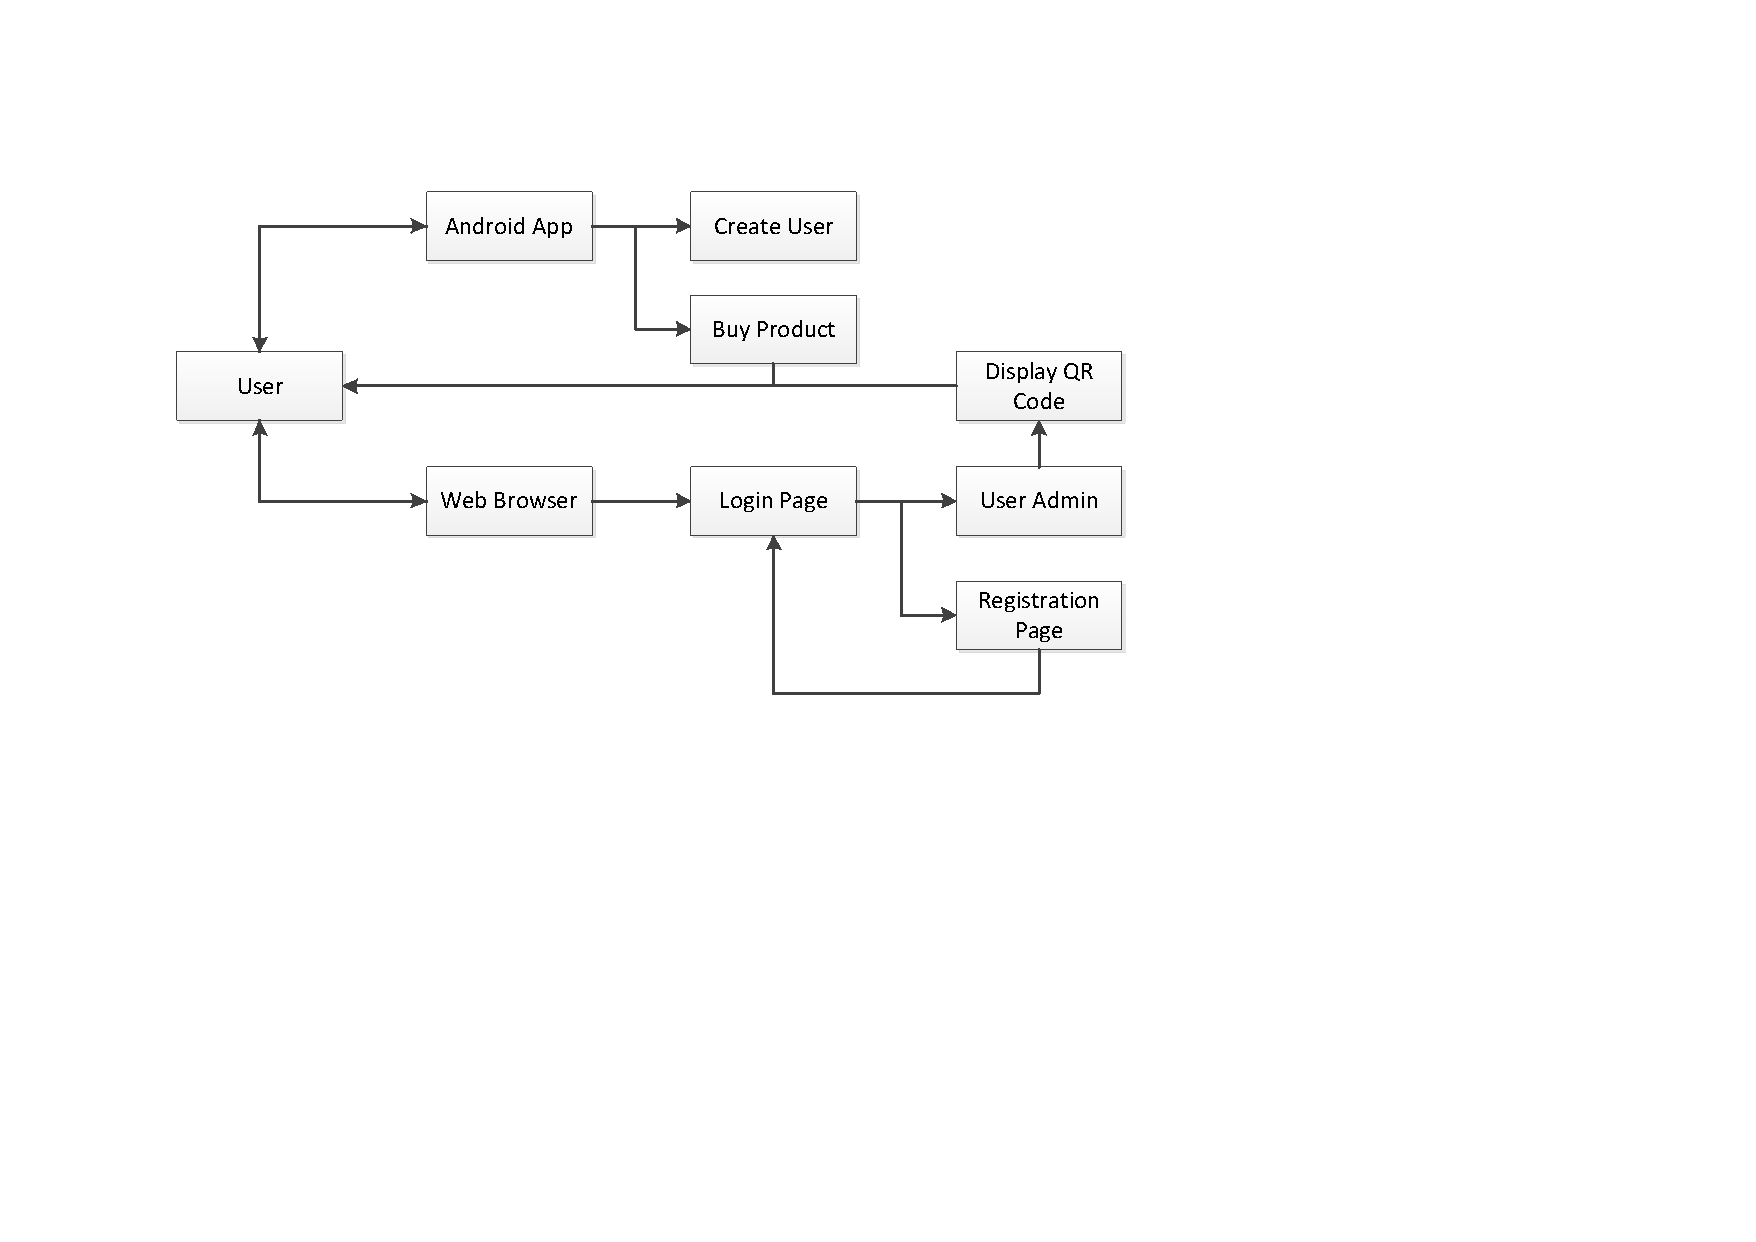
\includegraphics[clip=true, trim = 50 260 0 90,
 scale=0.7]{website_structure}
 \caption{The web server application structure.}
 \label{fig:website-apps}
\end{figure}

\subsubsection{display\_qrcode}

This application forms the core of the Quick Response Code (QR Code) payment handling
part of the server. See Fig. \ref{fig:disp-qrcode} for the process flow of
this application.

\begin{figure}
 \centering 
 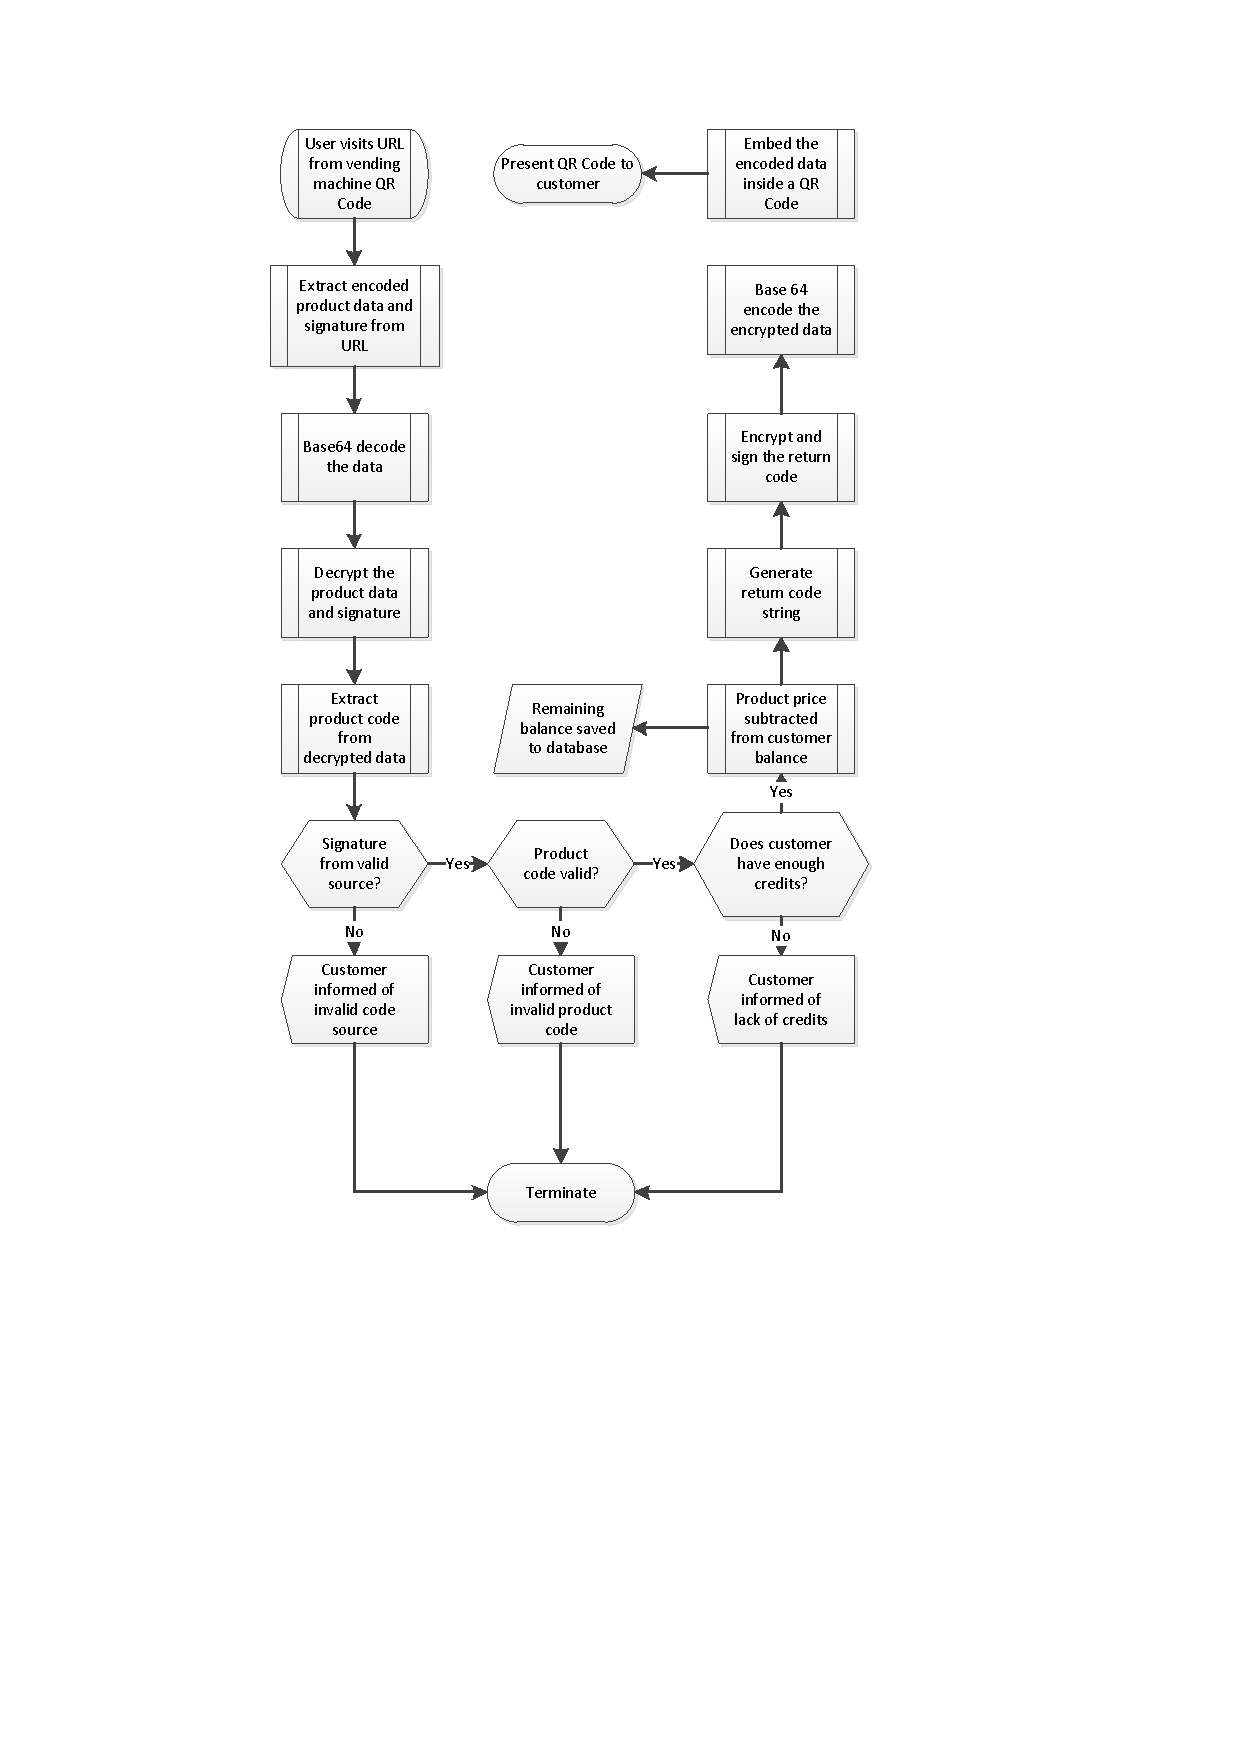
\includegraphics[clip=true, trim = 0 250 0 120,
 scale=0.7]{qrcode_processflow_server_bak}
 \caption{The display\_qrcode application process flow.} 
 \label{fig:disp-qrcode}
\end{figure}

Fig. \ref{fig:disp-qrcode} shows that the application first extracts the code
containing the product code and VM's signature from the Uniform
Resource Locator (URL) that the customer requested with his cellphone's web
browser. The application then proceeds to decode the product code from its base64
encoded format.

After successfully decoding the data, the application proceeds to decrypt the data and
signature with the ElGamal algorithm using the server's private key and the
VM's public key. Afterwards, following the security code scheme described in Sec.
\ref{sec:security-code-scheme}, it extracts the product code and challenge from the
decrypted string.

The application then checks to see whether the signature comes from a valid source (i.e.
one of the VMs using this system), whether the product code is
valid (i.e. the product is in the database) and whether the customer has enough
credits available. If either of these checks return false,
an error message is shown to the customer explaining what went wrong
and what the customer should do next.

If the checks were passed, the application proceeds to subtract the product cost from
the user's remaining balance. Following the security code scheme, the application then
generates the correct return code, encrypts and signs it with the vending
machine's public key and the server's private key, and encodes it in base64.
After this is completed, the application embeds this data into a QR Code, which is
displayed on the customer's cellphone screen.

\subsubsection{load\_money}

This application allows the customer to load money onto his account. At the moment it
makes use of faux money, meaning that the money loaded has no real-world value.
The customer can load a maximum of R1000.00 at a time onto his account. See Fig.
\ref{fig:load-money} for the process flow of this application.

\begin{figure}
 \centering 
 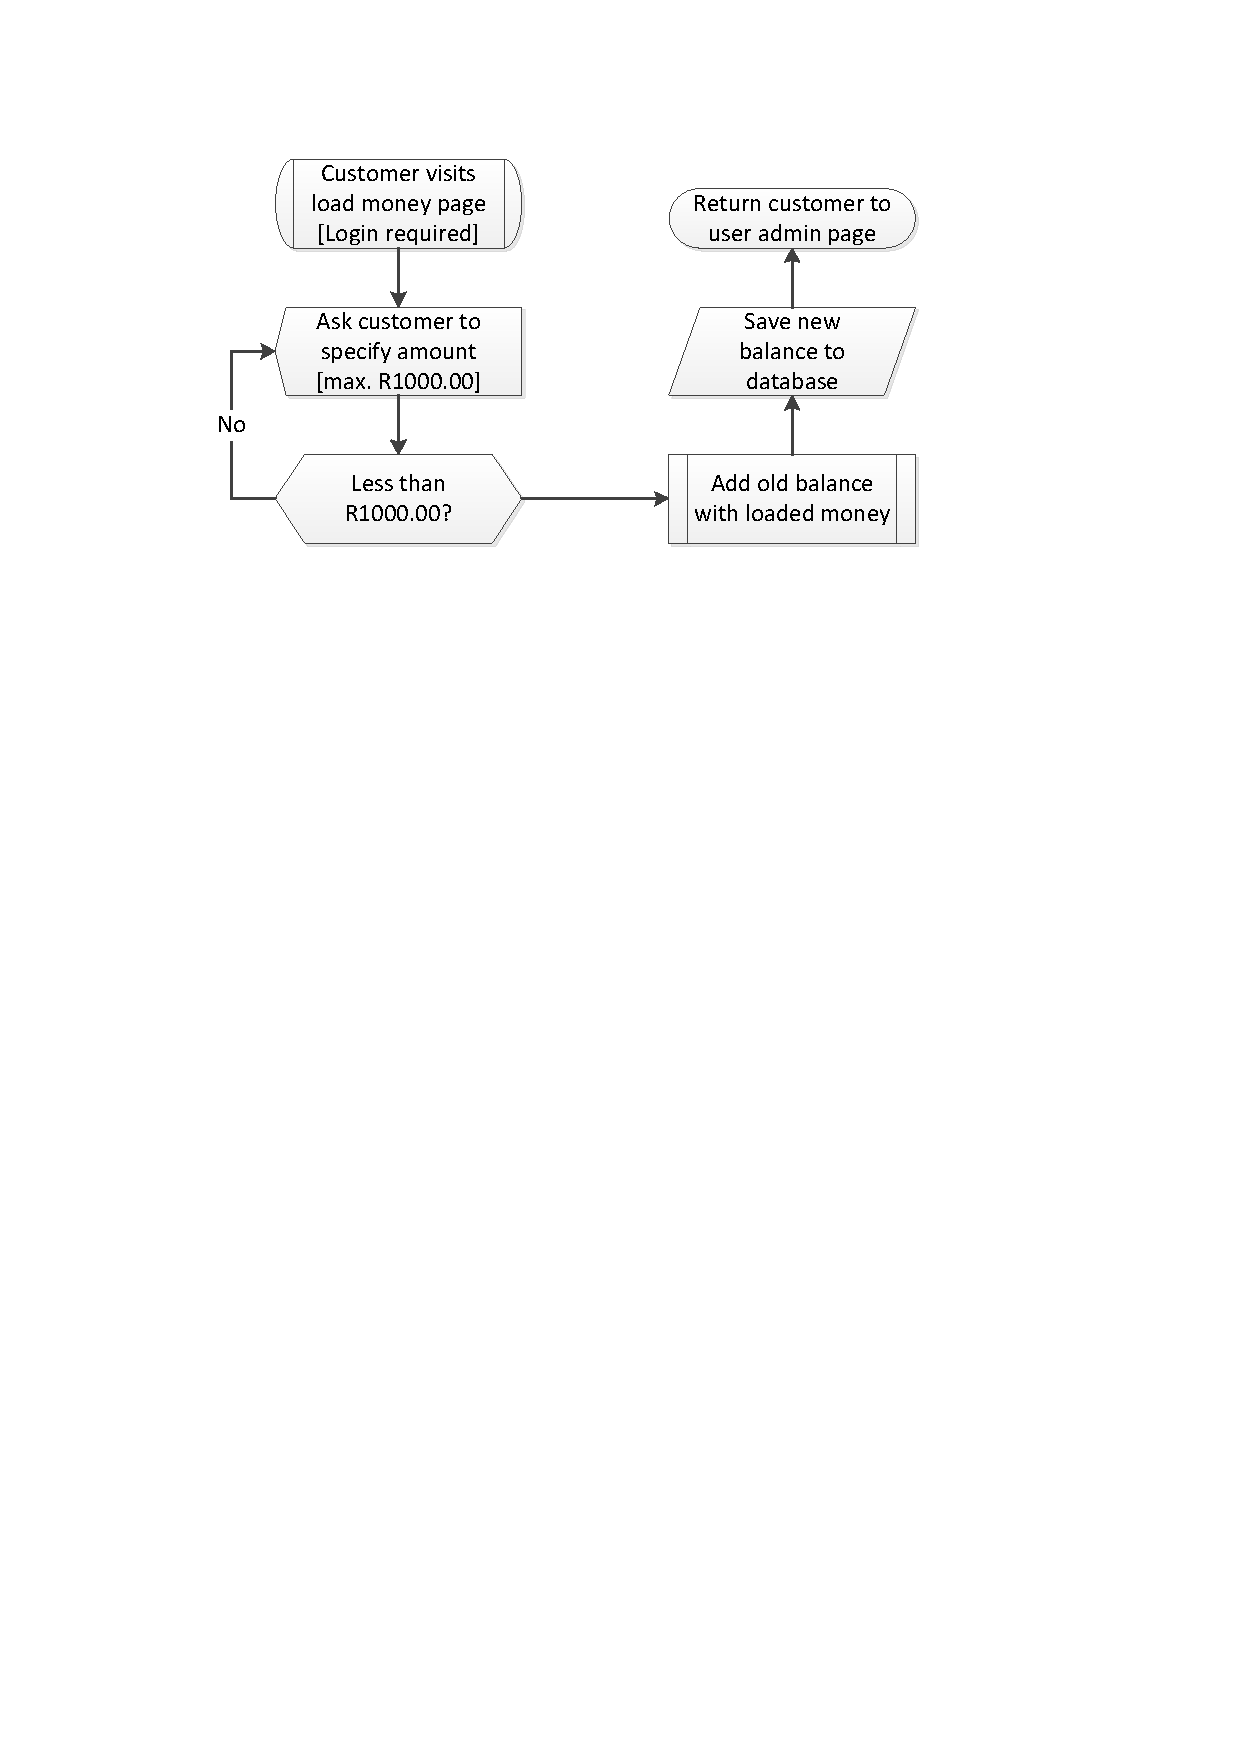
\includegraphics[clip=true, trim = 0 580 100 70,
 scale=0.7]{load_money}
 \caption{The load\_money application process flow.}
 \label{fig:load-money}
\end{figure}

\subsubsection{nfc}
\label{sec:app-nfc}

This application forms the core of the NFC payment handling part of the server. See Fig.
\ref{fig:nfc-process} for a detailed process flow diagram.

\begin{figure}
 \centering 
 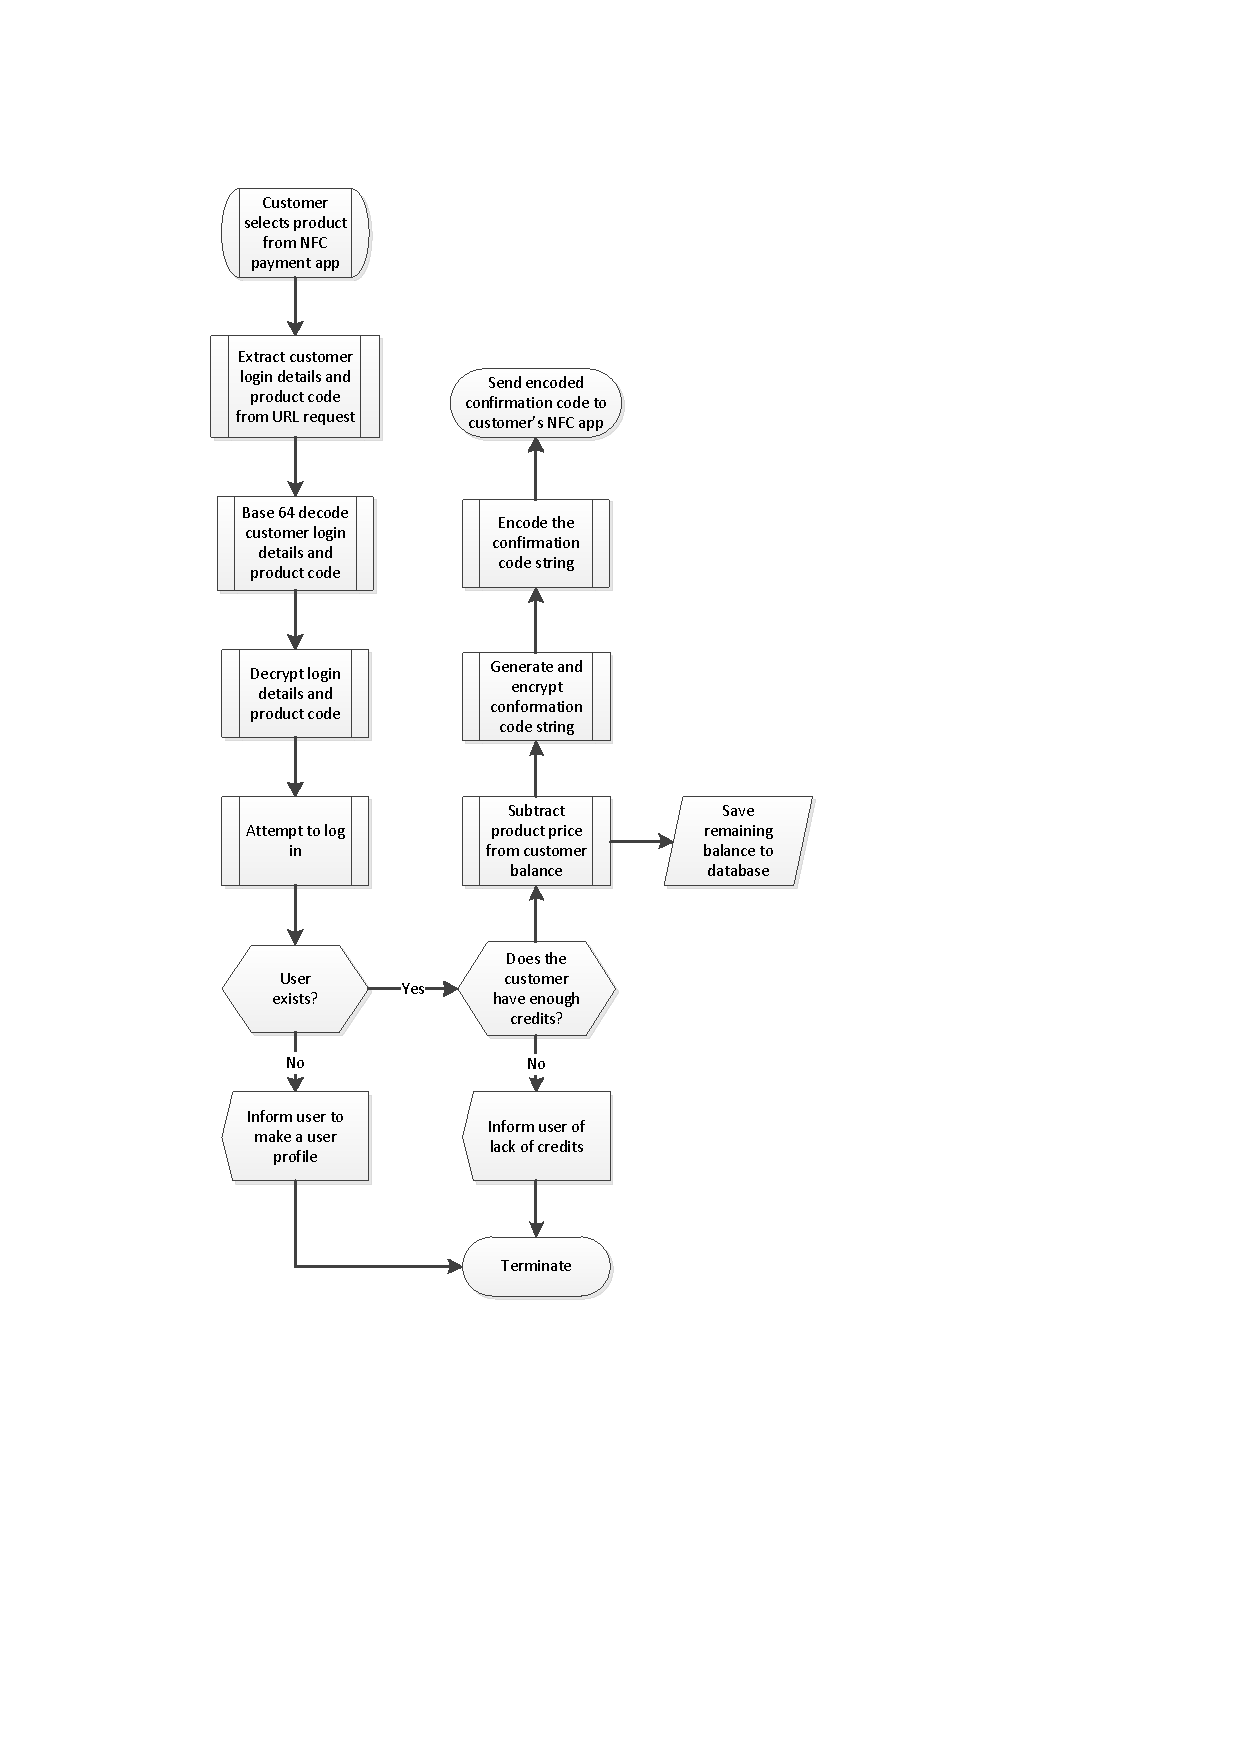
\includegraphics[clip=true, trim = 0 220 50 150,
 scale=0.7]{nfc_processflow_bak}
 \caption{The NFC application process flow.}
 \label{fig:nfc-process}
\end{figure}

Fig. \ref{fig:nfc-process} shows that the server first extracts the encrypted
customer login details and product code from the NFC application's URL request. These
codes are then decoded and decrypted using the RSA algorithm and the server's private key.

The user login details are then checked and verified using the server's user database. If this
check fails, the customer is given an error message and is asked to create a user profile.
If the check is passed, the server then checks to see if the customer has enough money
loaded onto his account. If this check fails, the customer is informed of his lack of
funds and is instructed to load more money. If the check is passed, the server subtracts
the product cost from the customer's balance and encrypts and encodes a confirmation
code, according to the security code scheme specified in Sec.
\ref{sec:security-code-scheme}. This code is then sent to the NFC application.

\subsubsection{nfc\_add\_user}

This application allows a customer using the NFC application to create a user profile for
himself. The server extracts the customer's login details from the URL request that the
NFC application sends to the server. These details are then saved to the database and is immediately available to be used by the new
customer. 

\subsubsection{register}

This application allows a new customer to register a new user profile with an internet
browser. This application is only accessible by a web browser and not by the NFC
application. However, a user registered with this application will be able to use the
same login details for the NFC application, and vice versa.

The application presents the user with a simple registration page which asks for a user
name, email and password. Using Django's built-in form support, the server handles the
POST request that is generated when the customer presses the `Continue' button. When this
is done, the customer's login details contained within the POST request is extracted and
saved into the user database.

\section{Vending Machine Program}

The vending machine's program runs the VM. It is responsible for
allowing the customer to select a product, to create a QR Code that redirects
the customer to the web server, to scan the customer's response QR Code, to
scan the customer's NFC/RFID request and to dispense the product after a successful
transaction.

The whole program is based on Python and designed to be used by a Raspberry Pi
microcomputer. To simplify the program, it is split into separate subprograms. These
subprograms, called scripts, are discussed in this section. The complete
program structure and its inter-script interfaces can be seen in Fig.
\ref{fig:vm_prog_strcture}.

\begin{figure}
 \centering 
 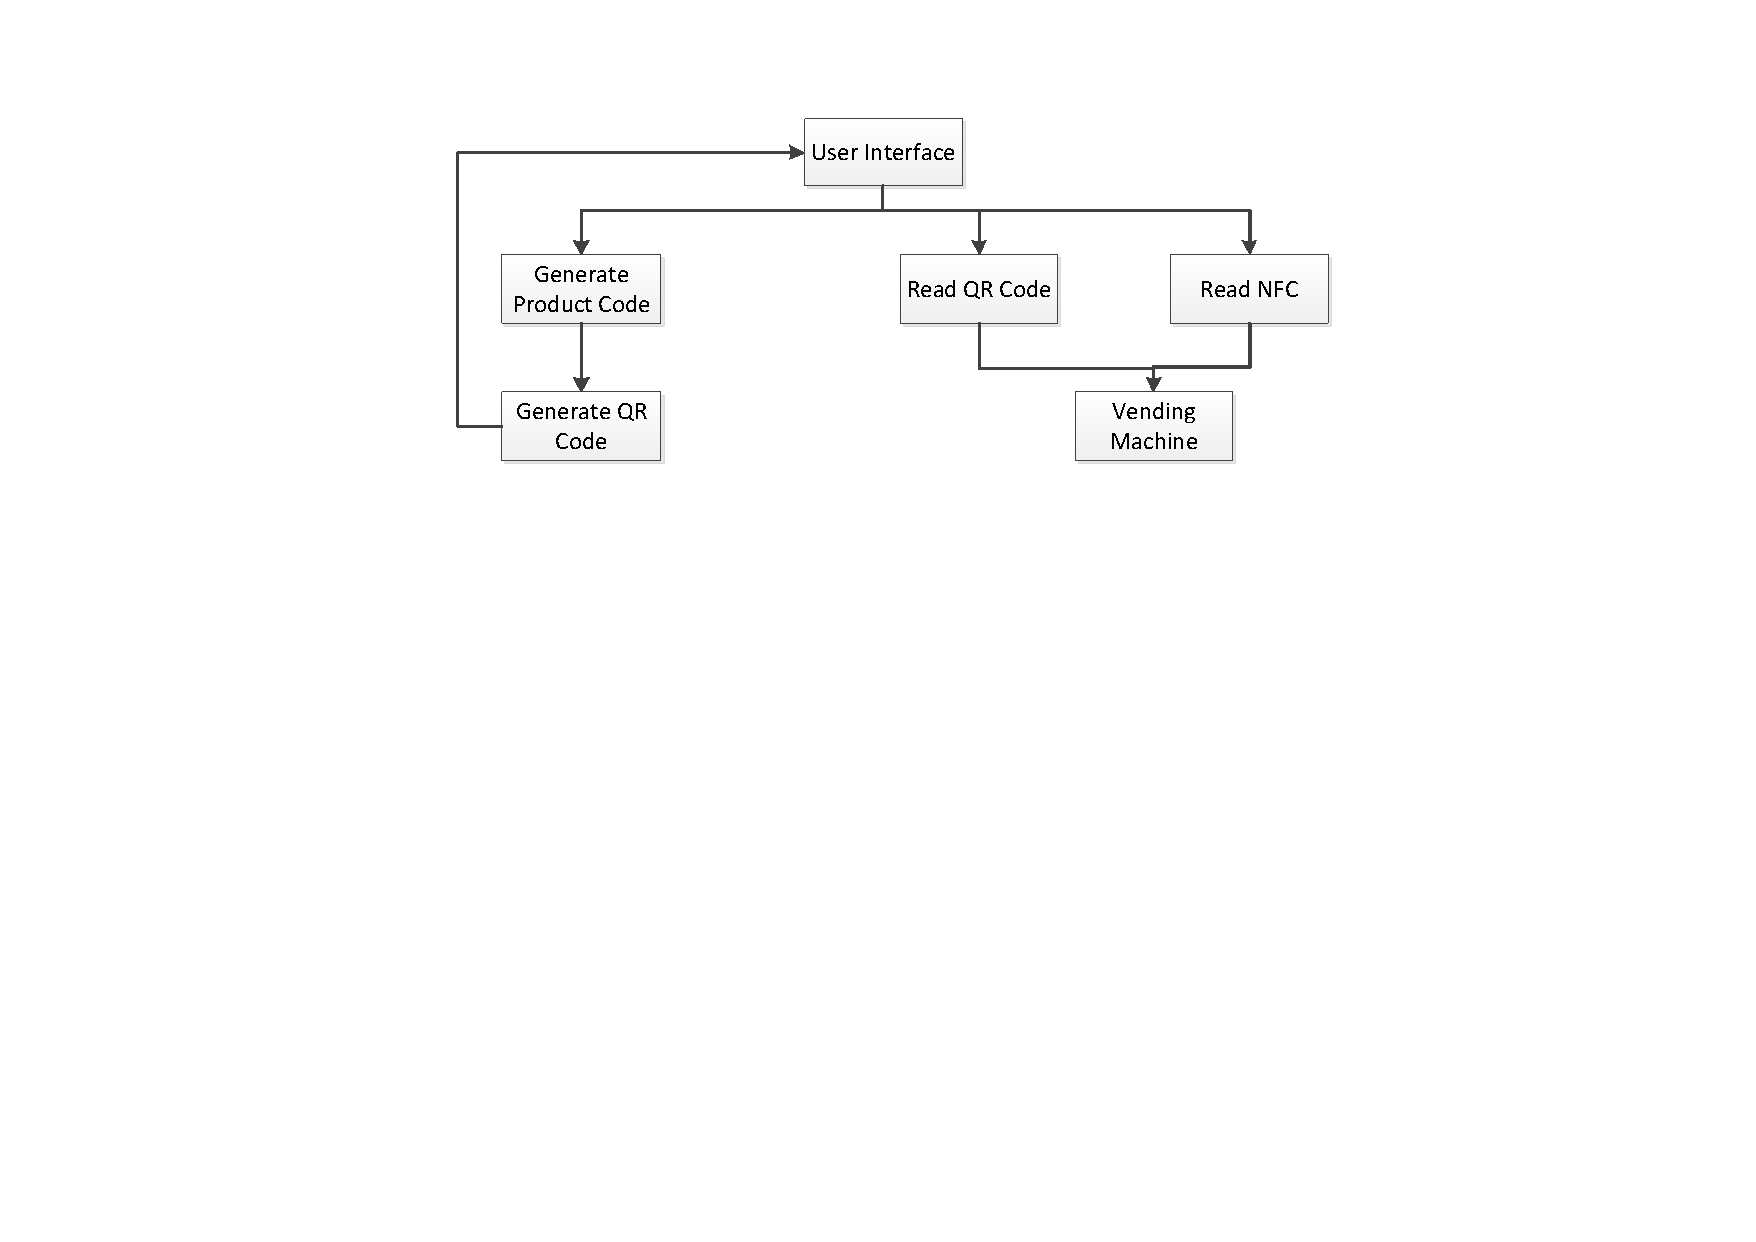
\includegraphics[clip=true, trim = 120 370 0 50,
 scale=0.7]{vending_machine_program_structure}
 \caption{The vending machine's program structure.}
 \label{fig:vm_prog_strcture}
\end{figure}

\subsection{User Interface}

To allow the customer to select a product, a Graphical User Interface (GUI) was
created. The GUI was made using the WX Python GUI toolkit
[\cite{website:wx-python}].
See Fig. \ref{fig:gui-screenshot} for a screenshot of the
GUI.

\begin{figure}
 \centering 
 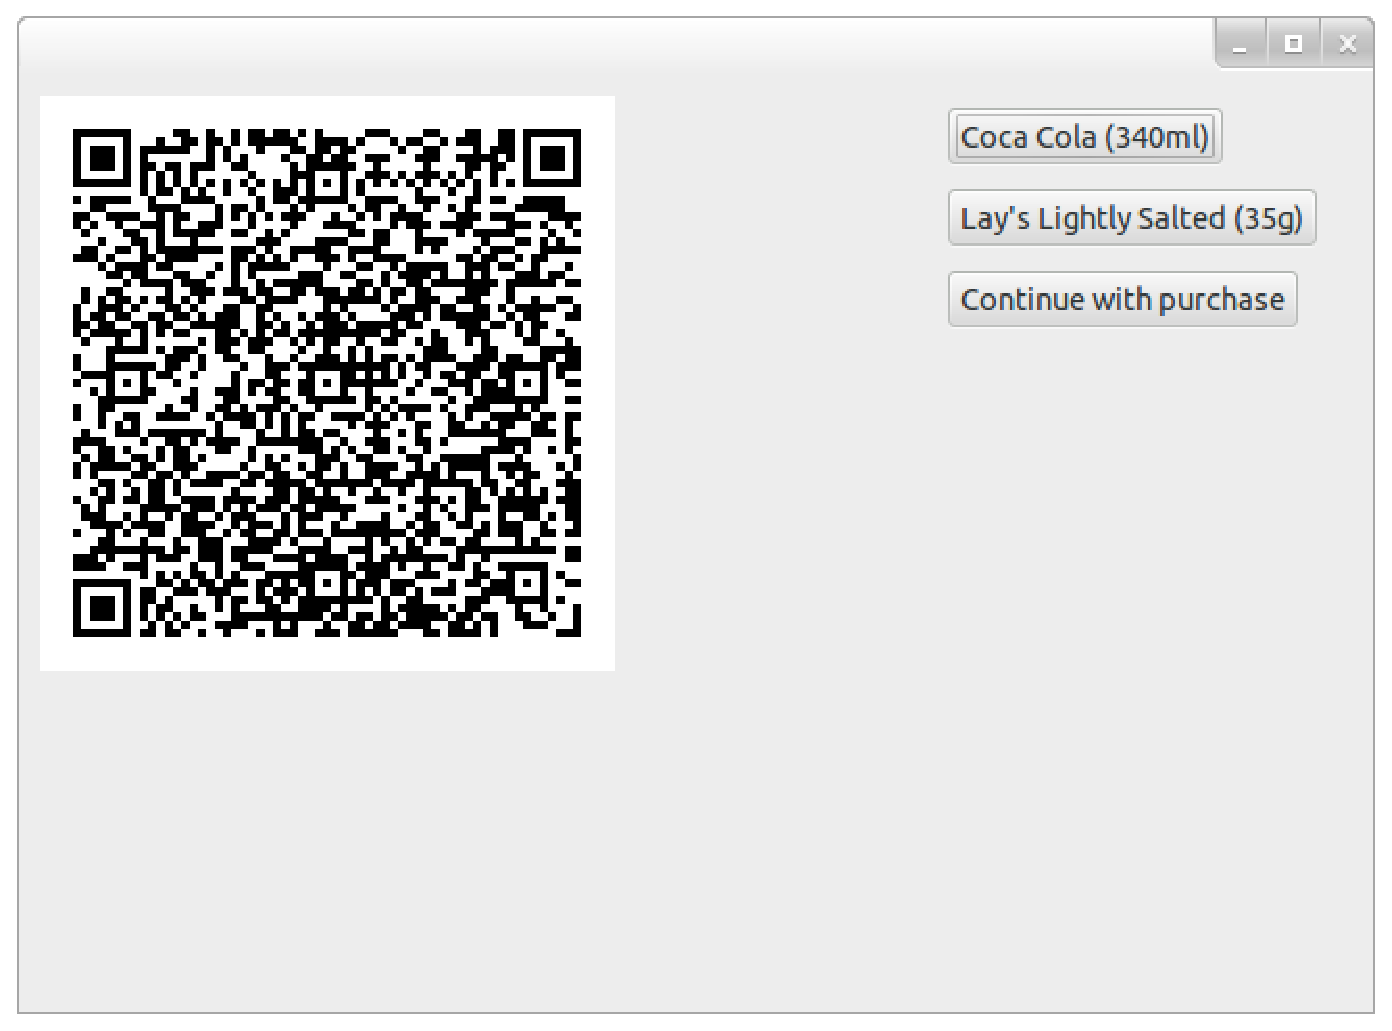
\includegraphics[clip = true, trim = 190 370 0 350, scale=2]{gui_screenshot}
 \caption{A screenshot of the user interface.}
 \label{fig:gui-screenshot}
\end{figure}

As can be seen from Fig. \ref{fig:vm_prog_strcture}, the GUI script is
responsible for calling the encryption script and the QR Code generation script.
It is also responsible for displaying the QR Code, to handle transactions from
the Android NFC application and to activate the correct motor inside the vending
machine. 

\subsection{Generating a Product Code}

After the customer selects which product to buy from the GUI, the
encrypt\_elgamal script is called. This script is responsible for generating the
random hex character string, in accordance with the security scheme described in
Sec. \ref{sec:security-code-scheme}, encrypting, signing and encoding the
string in base64 and embedding the random string inside a URL that points to the web
server. This URL is then sent to the generate\_qrcode script described in Sec.
\ref{sec:gen-qrcode}. See Fig. \ref{fig:gen-prod-code-processflow} for a detailed process
flow diagram.

\begin{figure}
 \centering 
 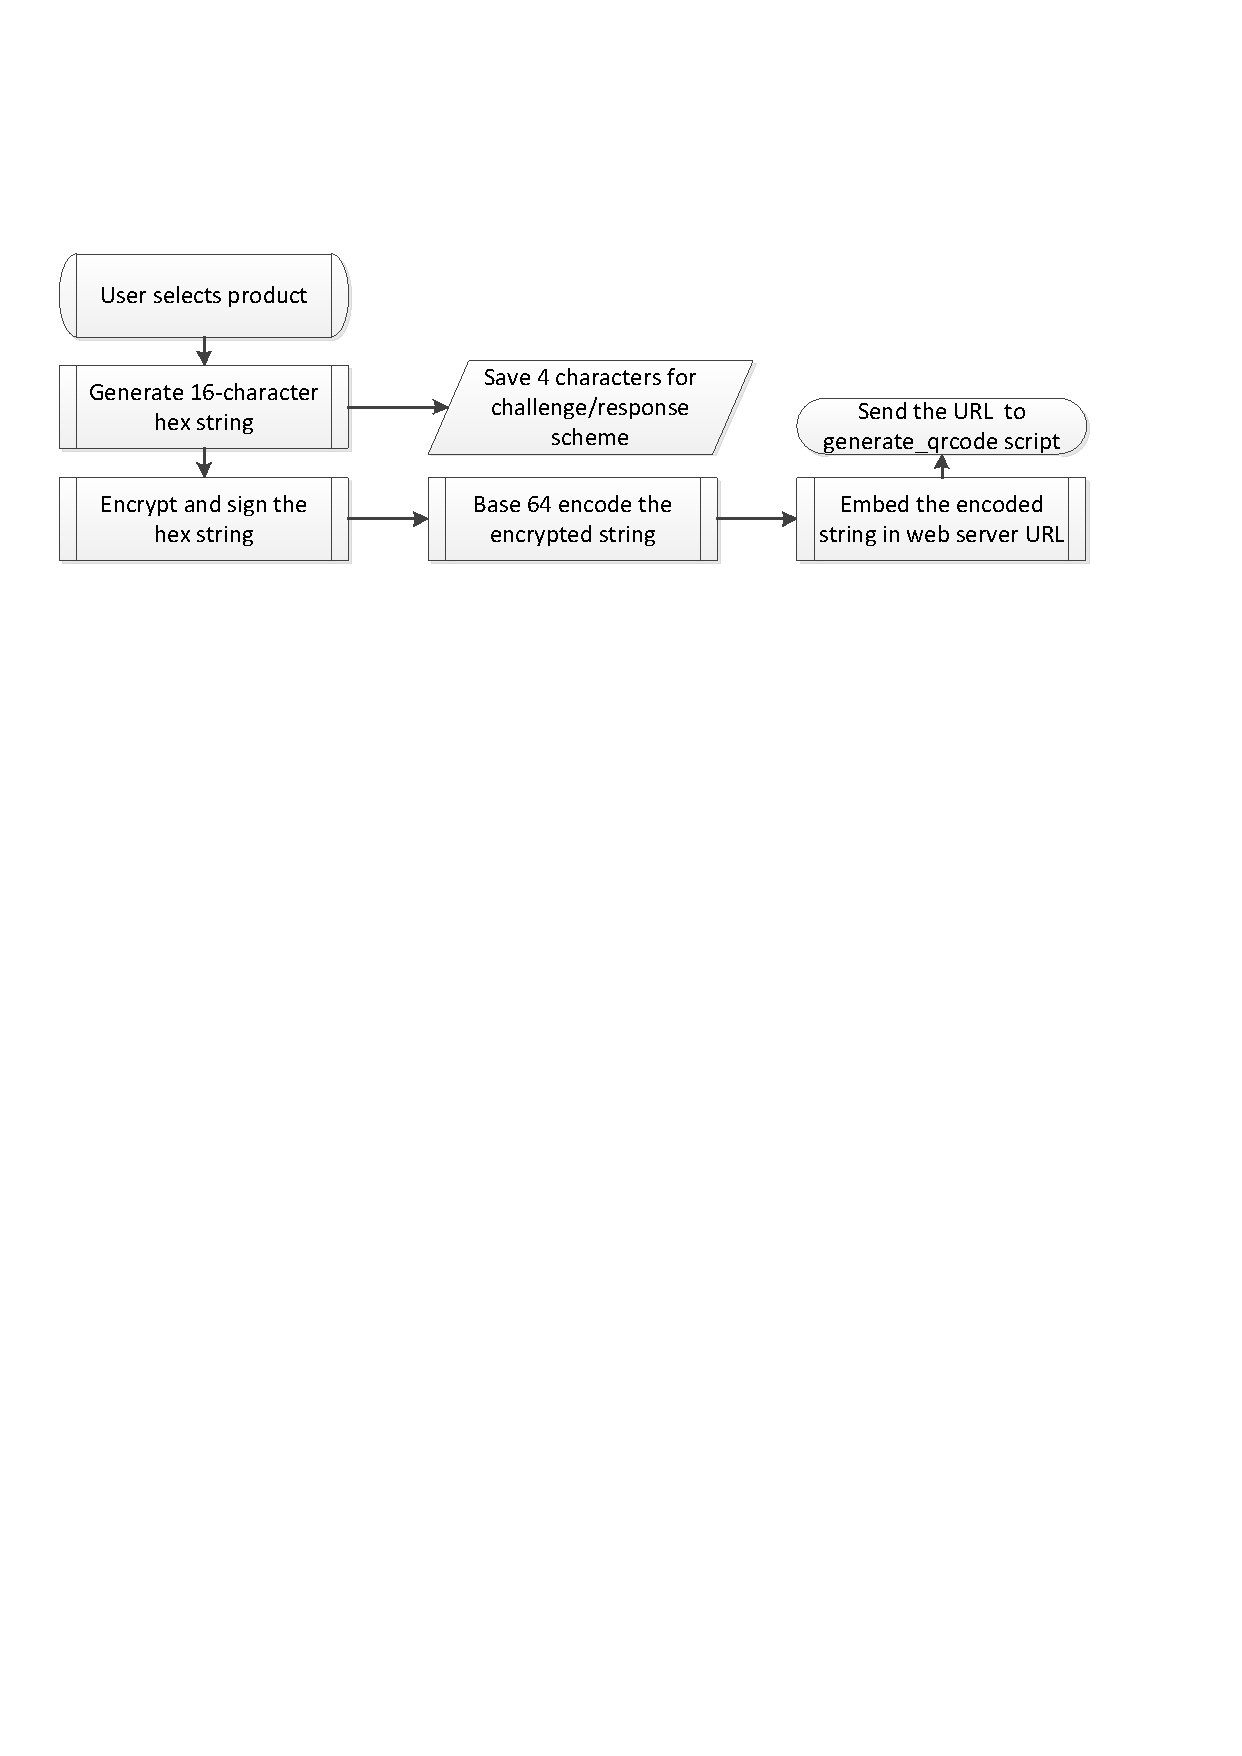
\includegraphics[clip=true, trim = 0 570 50 120, scale=0.7]{gui_processflow}
 \caption{The GUI process flow.}
 \label{fig:gen-prod-code-processflow}
\end{figure}

\subsection{Generating a QR Code}
\label{sec:gen-qrcode}

After the encrypt\_elgamal script has been run, the generate\_qrcode script is
called. This script is responsible for embedding the URL received from the
encrypt\_elgamal script into a QR Code. This is done by using a qrcode module
for Python, called qrcode [\cite{website:qrcode-generator}].

\subsection{Reading a QR Code}

After the customer has received his verification QR Code from the server, the customer
may presses `Continue with purchase' button. When this is done, the read\_qrcode script is
run. This script is responsible for reading the customer's QR Code via a webcam,
extracting the data from the scanned image, decrypting the data and verifying the
transaction. See Fig. \ref{fig:read-qrcode-processflow} for the process flow diagram.

\begin{figure}
 \centering 
 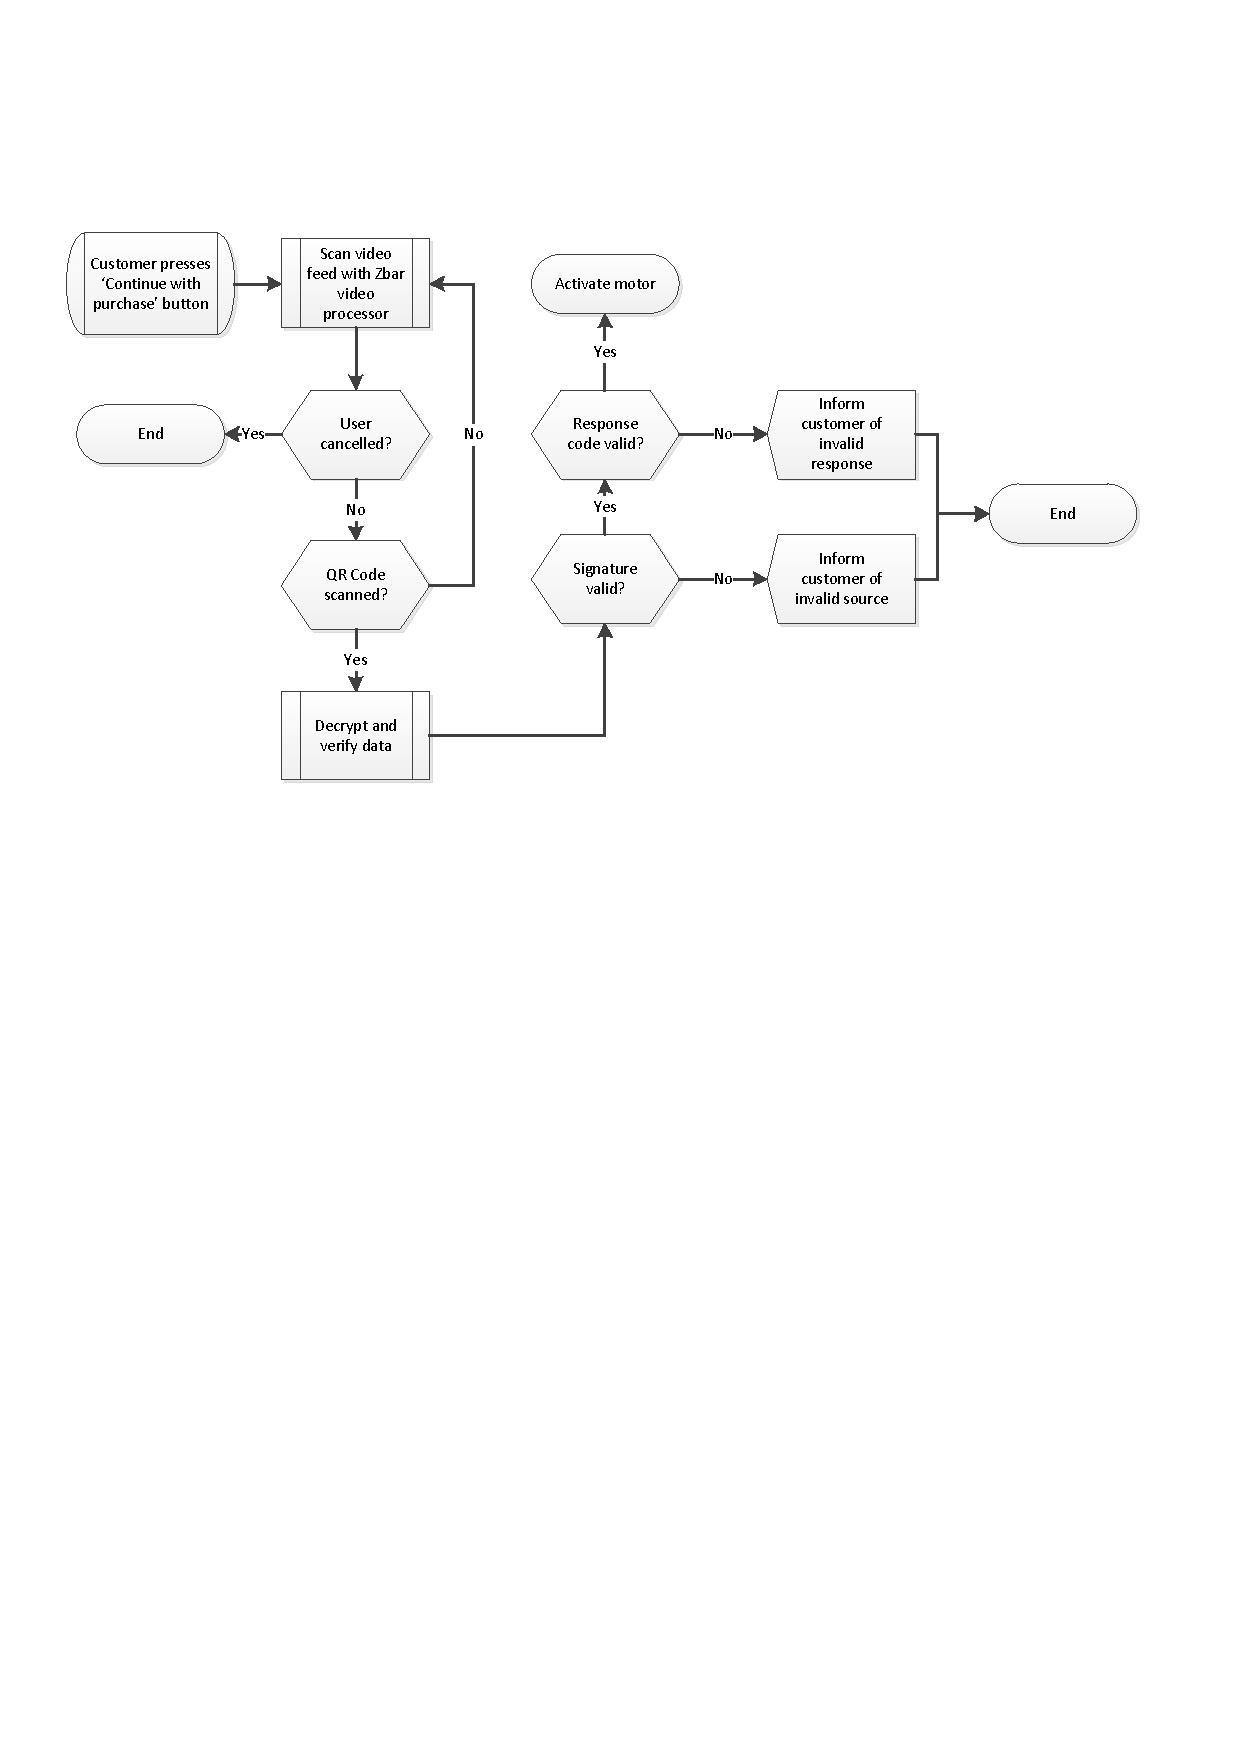
\includegraphics[clip=true, trim = 0 400 50 80, scale=0.75]{read_qrcode_processflow}
 \caption{The generate\_qrcode script process flow.}
 \label{fig:read-qrcode-processflow}
\end{figure}

As seen from Fig. \ref{fig:read-qrcode-processflow}, as soon as the `Continue
with purchase' button is pressed, a ZBar image processor is created
which scans a webcam video feed for a QR Code. The image processor runs until the user
cancels it or it scans a QR Code. 

After the ZBar processor has scanned a QR Code, it sends the retrieved data to
be decrypted and verified with the ElGamal algorithm, using the VM's
private key and the server's public key. If the signature is valid and the data
contains a valid response and product code, the script activates the correct
motor and the customer receives his product. 

\subsection{Near Field Communication}

If the customer opts to purchase a product with the Android NFC application, the NFC
script is run. This script is based on an example script included in the nfcpy package and is written by nfcpy's creator, Stephen
Tiedemann [\cite{website:nfcpy}]. This example script, called snep\_test\_server.py,
connects the Pi to the NFC controller chip, polls the chip for a Simple NFC Data Exchange Format
Exchange Protocol (SNEP) message, and when a SNEP message is read, it extracts the data
in the message and presents it to the programmer for further processing and manipulation.
This script allows the VM to extract SNEP messages from any source that
follows the NFC Forum's standards [\cite{website:nfc-forum}]. For this project, an
Android application was written specifically for this purpose.

After the data is extracted from the NFC source, the script decrypts the data
using the RSA algorithm and the VM's private key. The vending
machine then checks the NFC message's response code. If the response code is valid, the
script then activates the correct motor to dispense the product to the customer.

\section{Android Application}
\label{sec:nfc-android-app}

An Android NFC application was made for this project. It allows a customer to buy a
product from the application's product menu and to complete the purchase by tapping
his phone against the VM's NFC receiver.

The application is divided up into three activities (Android's technical term for what
is essentially a different window of the application).  These activities, their design and
significance are discussed in this section. See Fig. \ref{fig:nfc_app_structure} for a
diagram of the application's inter-activity interactions.

\begin{figure}
 \centering 
 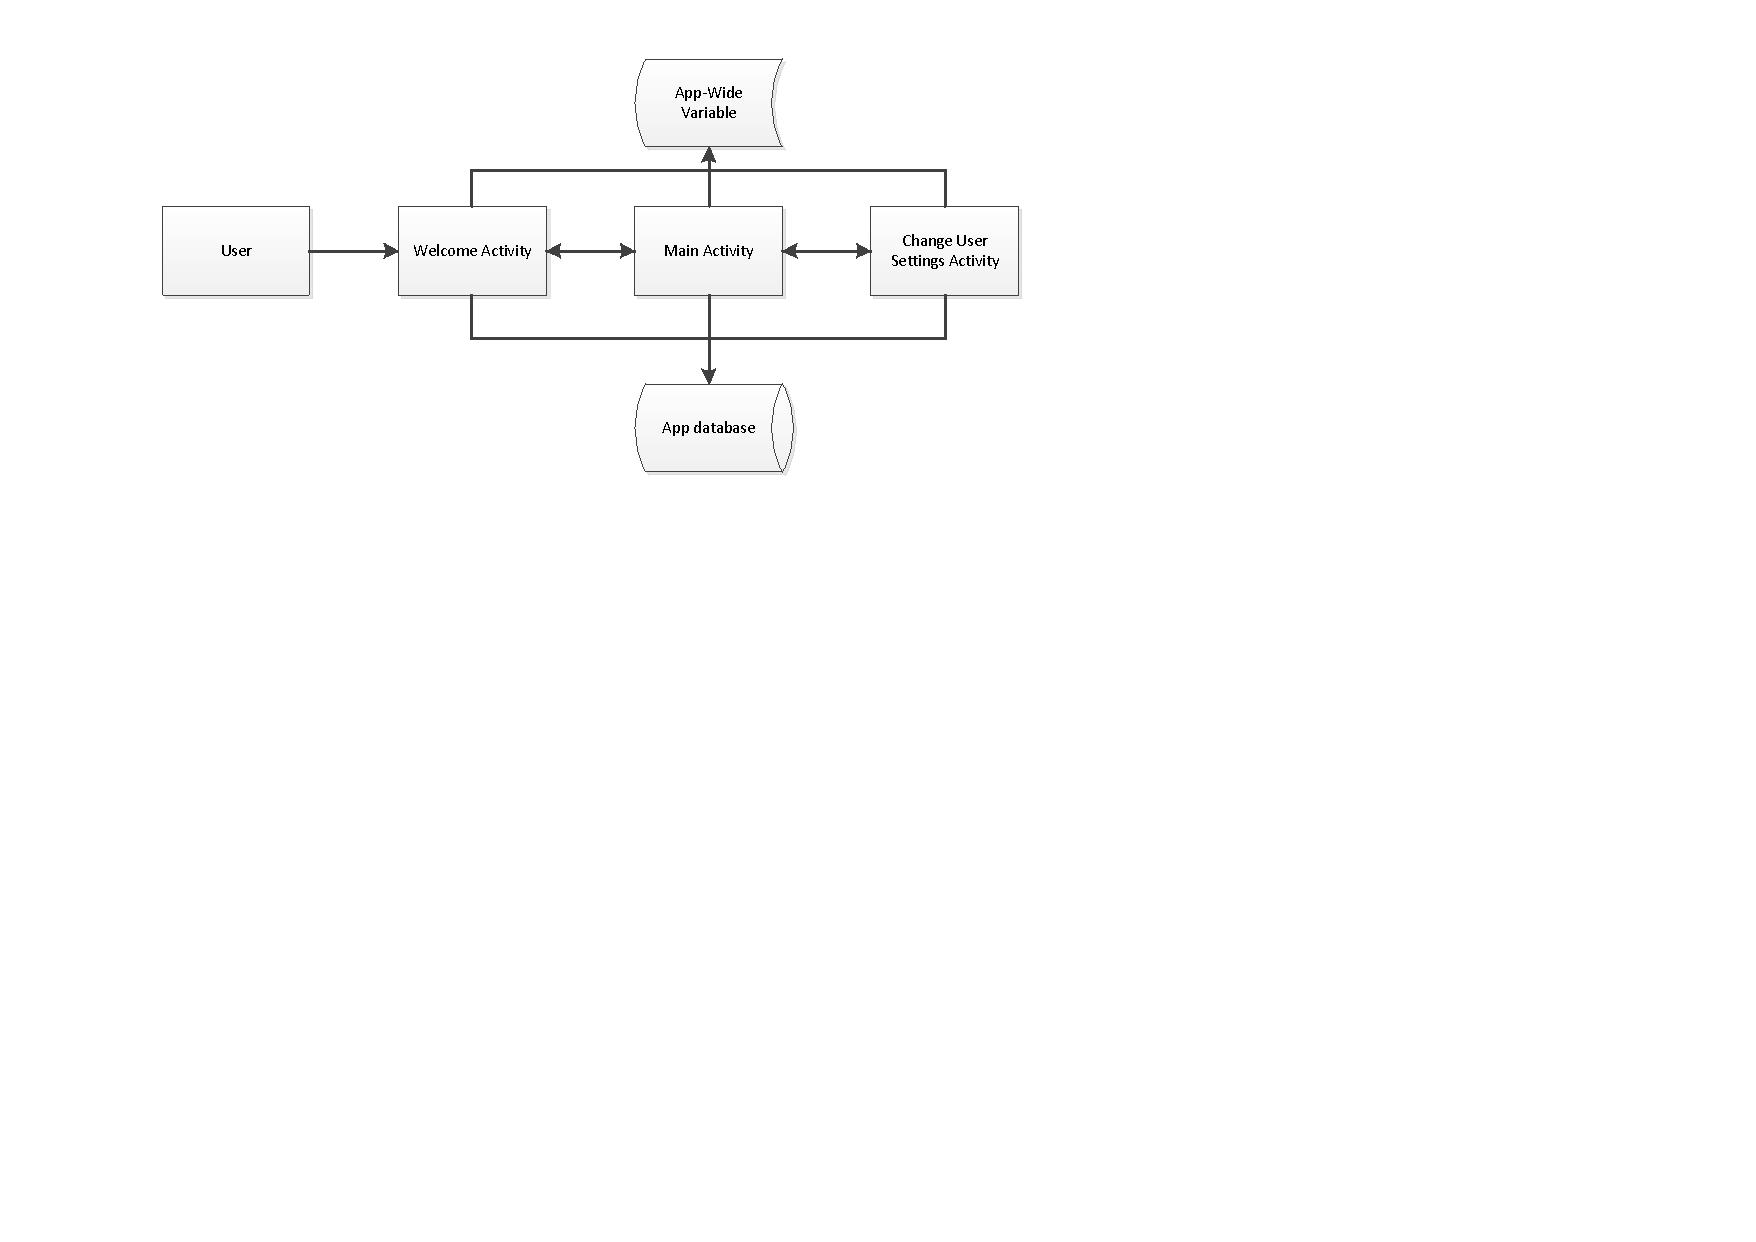
\includegraphics[clip = true, trim = 40 410 0 20,
 scale=0.7]{app_structure}
 \caption{The Android NFC application structure.}
 \label{fig:nfc_app_structure}
\end{figure}

\subsection{Welcome Screen}

This activity is called when the application is opened. This
activity's process flow can be seen in Fig. \ref{fig:app-welcomescreen}.
Fig. \ref{fig:welcomescreen-screenshot} shows a screenshot of the welcome
screen.

\begin{figure}
 \centering 
 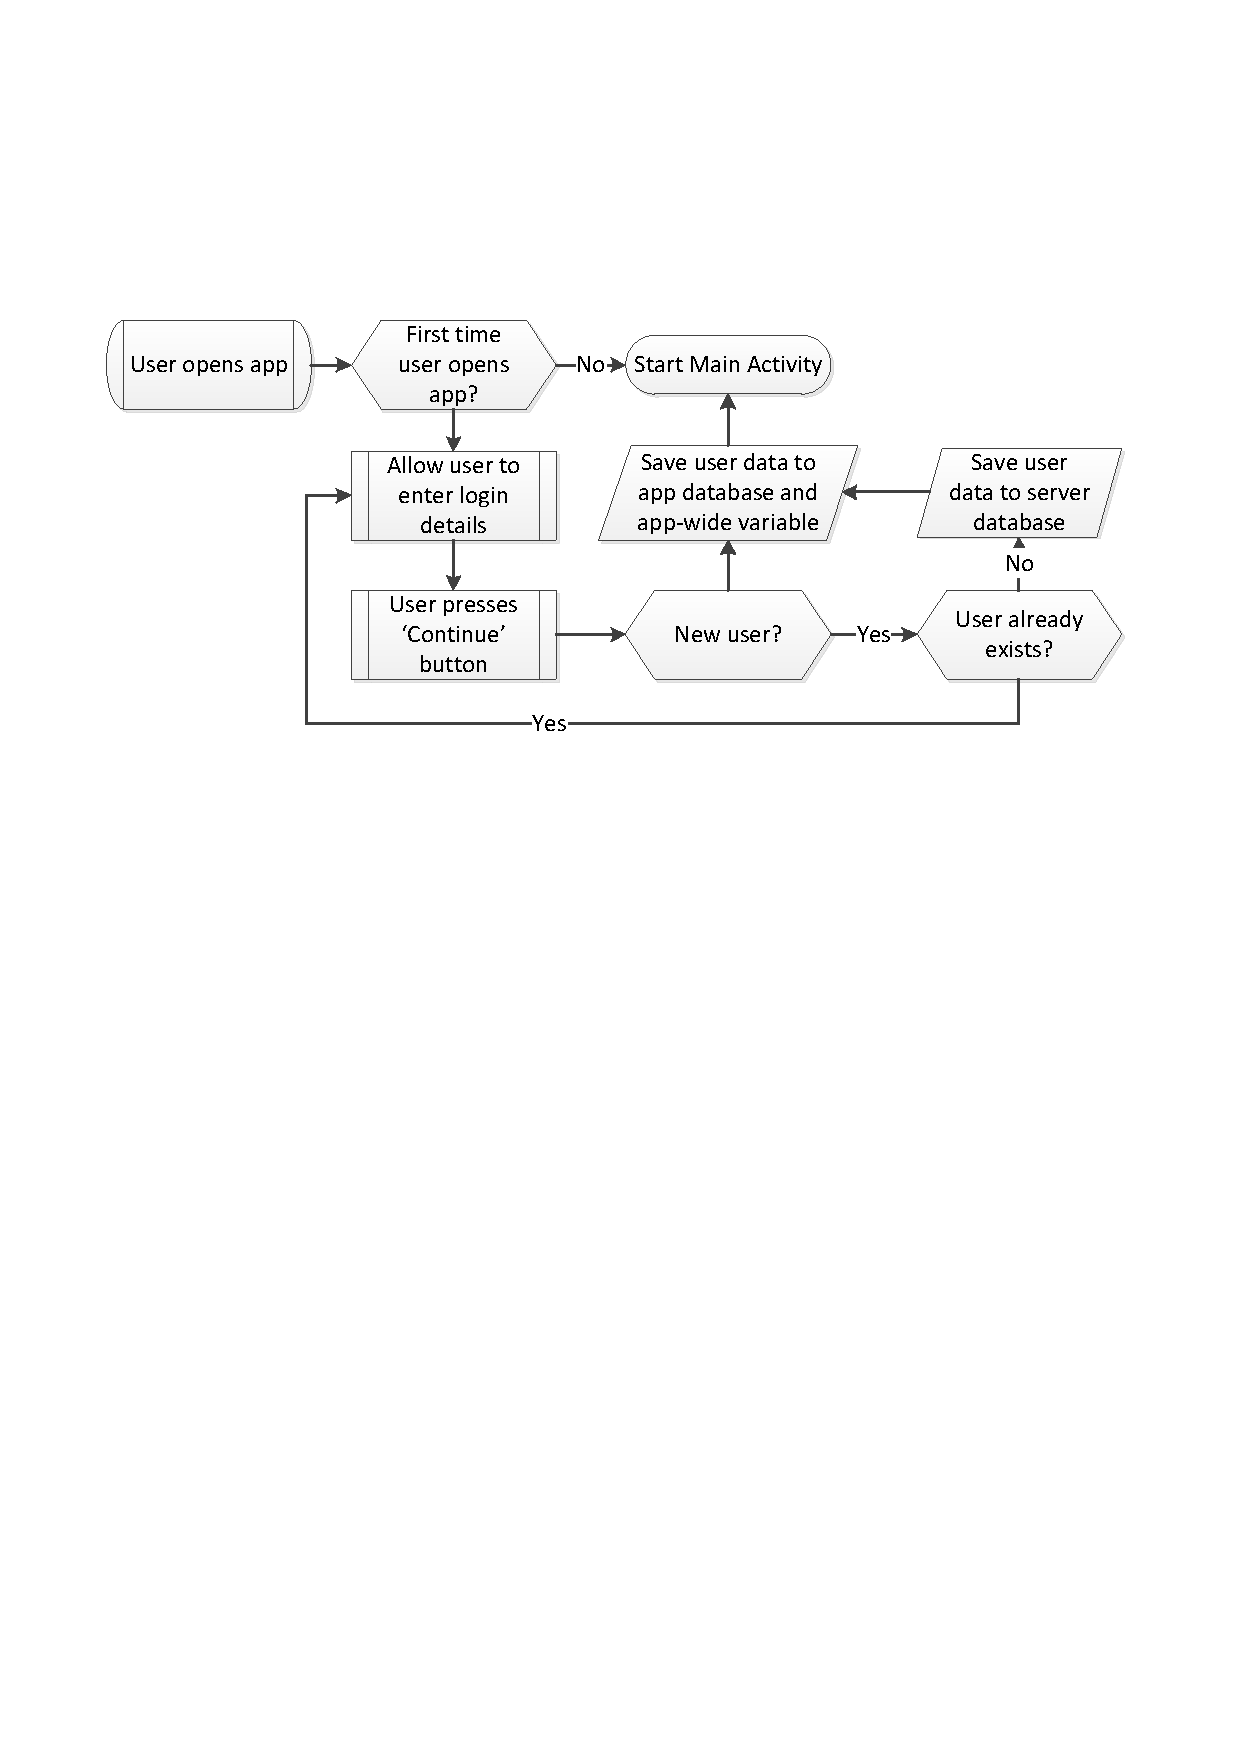
\includegraphics[clip = true, trim = 30 490 0 150,
 scale=0.75]{welcome_screen_processflow}
 \caption{The Android NFC application welcome screen.}
 \label{fig:app-welcomescreen}
\end{figure}

\begin{figure}
 \centering 
 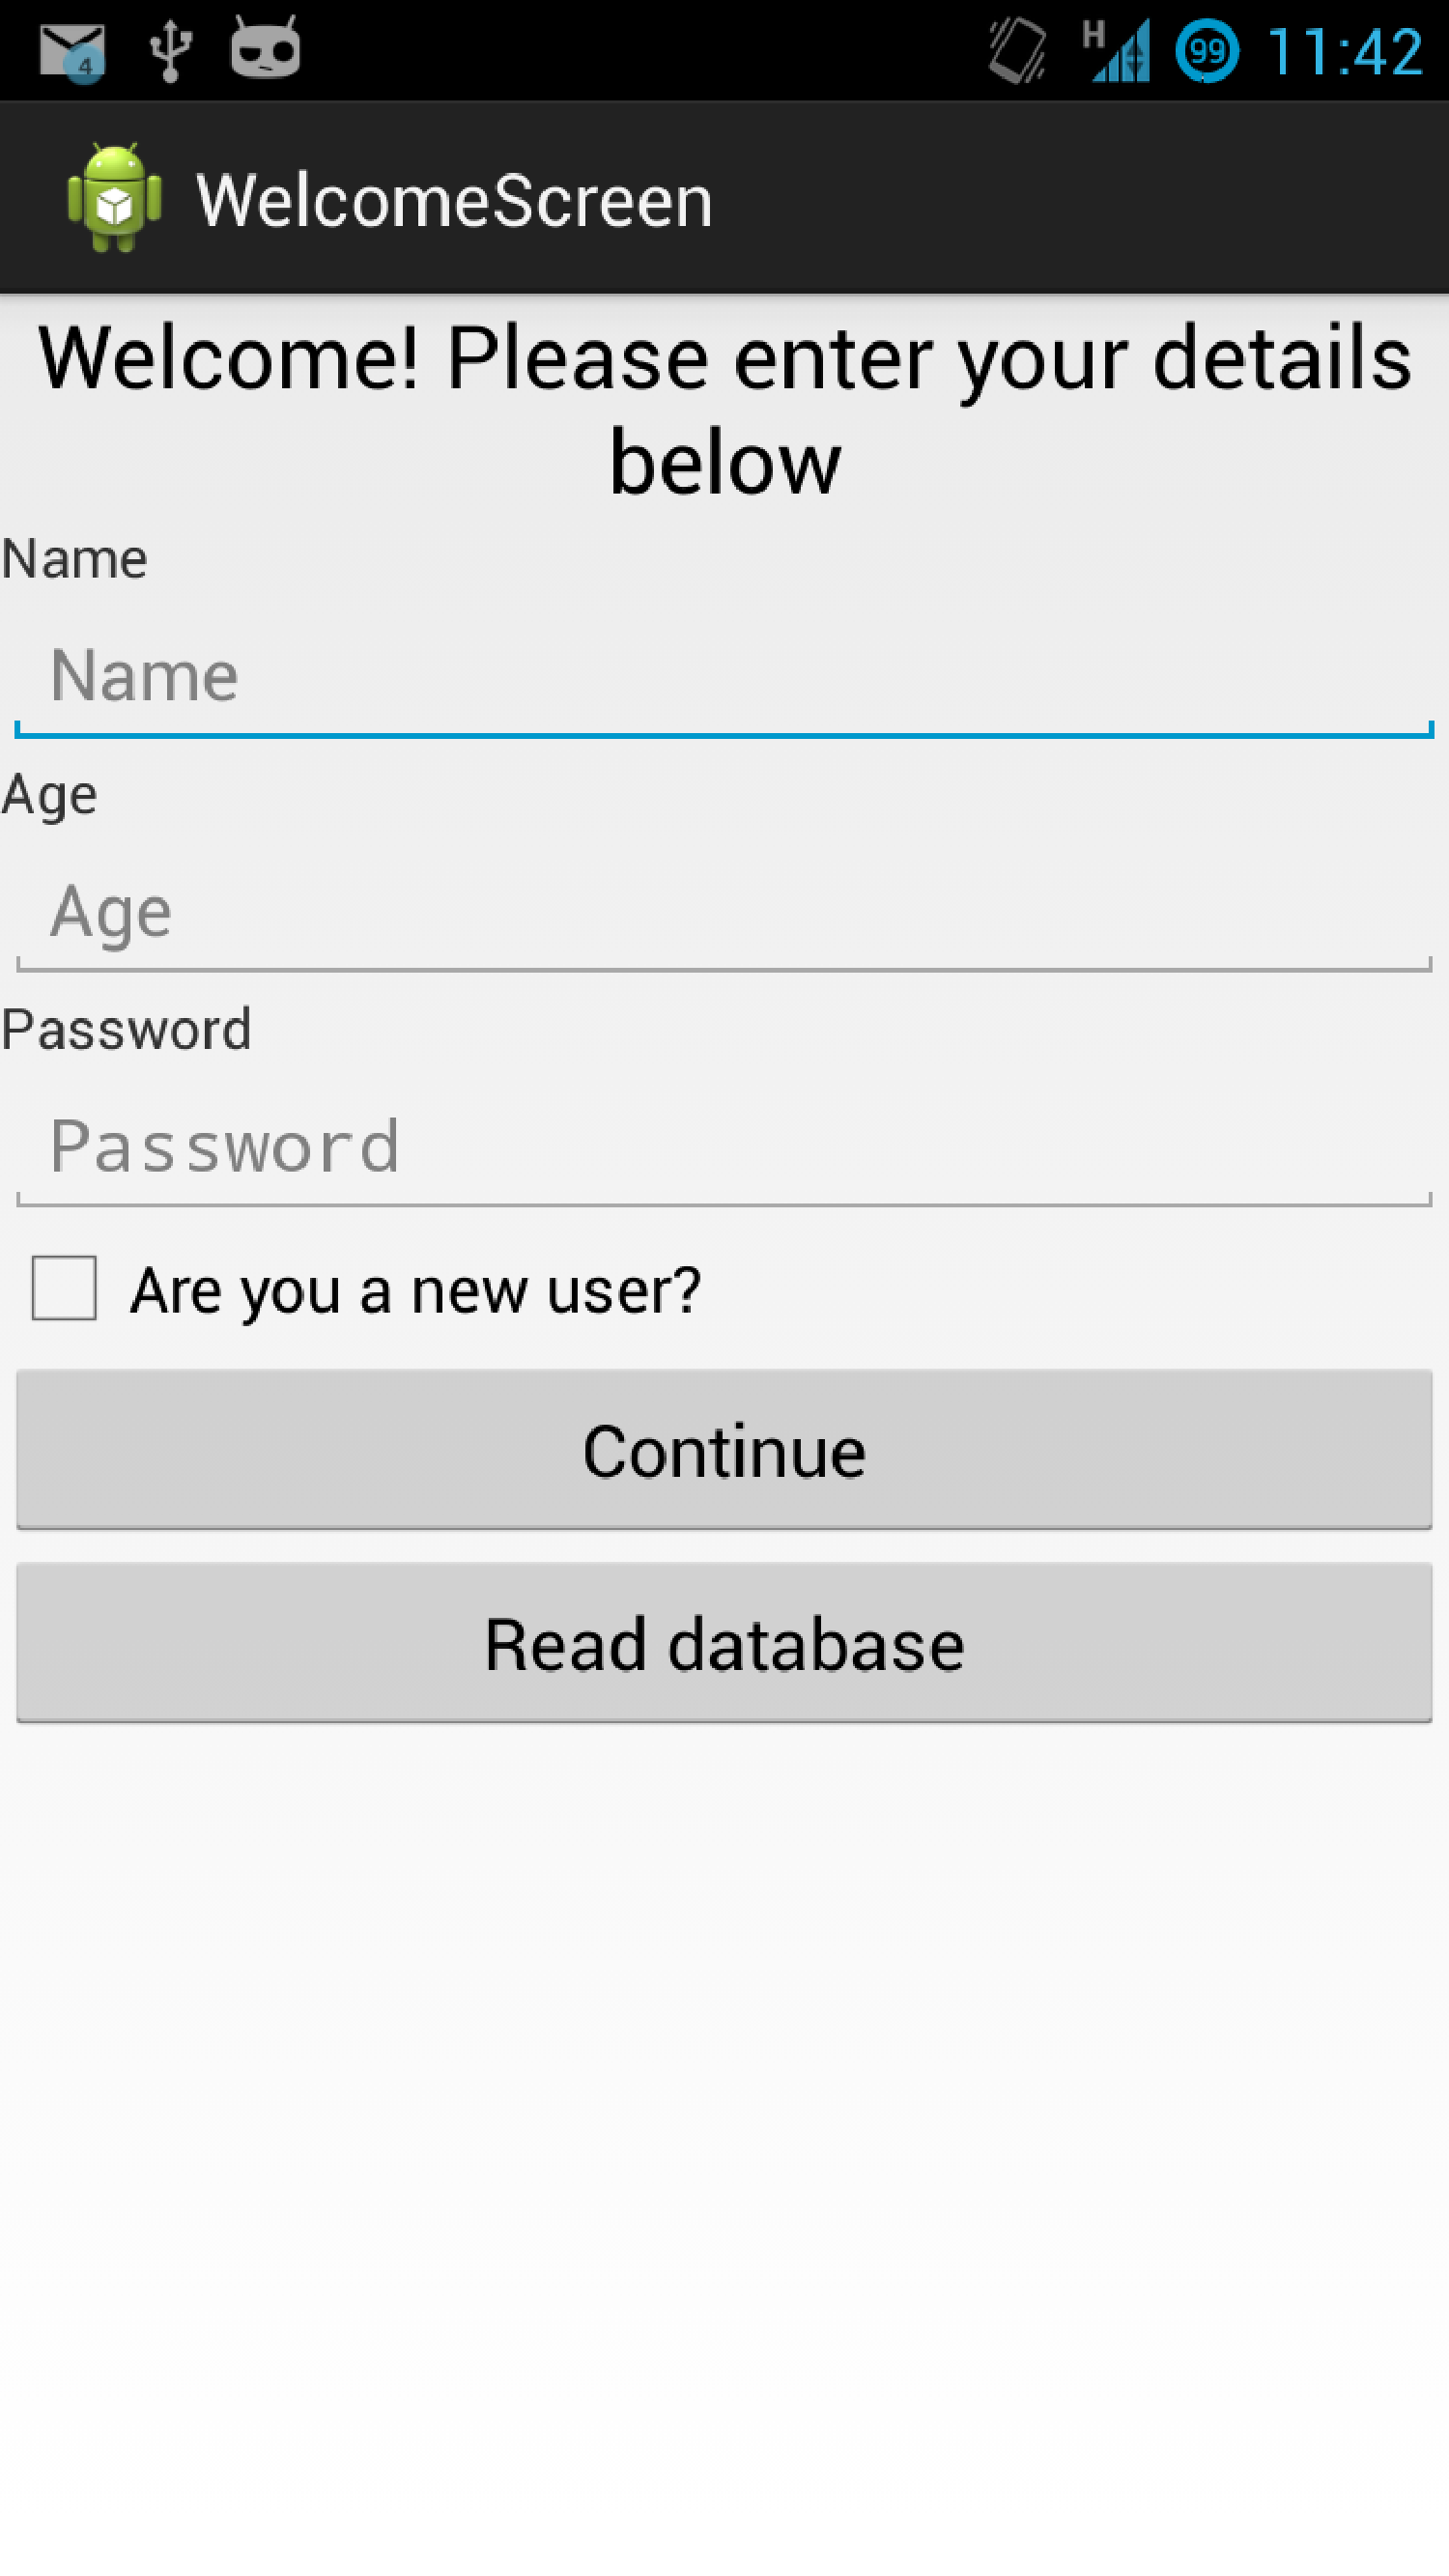
\includegraphics[clip = true, trim = 0 370 0 60, scale=0.2]{welcome_screen}
 \caption{A screenshot of the application's welcome screen.}
 \label{fig:welcomescreen-screenshot}
\end{figure}

As seen from Fig. \ref{fig:app-welcomescreen}, the
activity first checks to see whether it is the first time the user opens the
application. If it is not, the activity goes on to the Main Activity. Otherwise, it allows
the user to either sign in with an existing profile or create a new one.

When the user signs into an existing profile, the login details he provides
is stored in a database inside the application. When this is done, it
makes the login information persistent throughout the lifetime of the application. These
details are also saved into an application-wide variable. This variable is used to make
the application more efficient by not having to read the database as often. This variable
is only active while the application is running in the foreground or background. The
login details saved here are used later by the application's other activities.

\subsection{Change User Settings}

The Change User Settings activity allows the user to change his login
details that are saved in the database and the application-wide variable. See Fig.
\ref{fig:change-user-settings} for a process flow diagram for this
activity. Fig. \ref{fig:change-settings-screenshot} shows a screenshot of this
activity.

\begin{figure}
 \centering 
 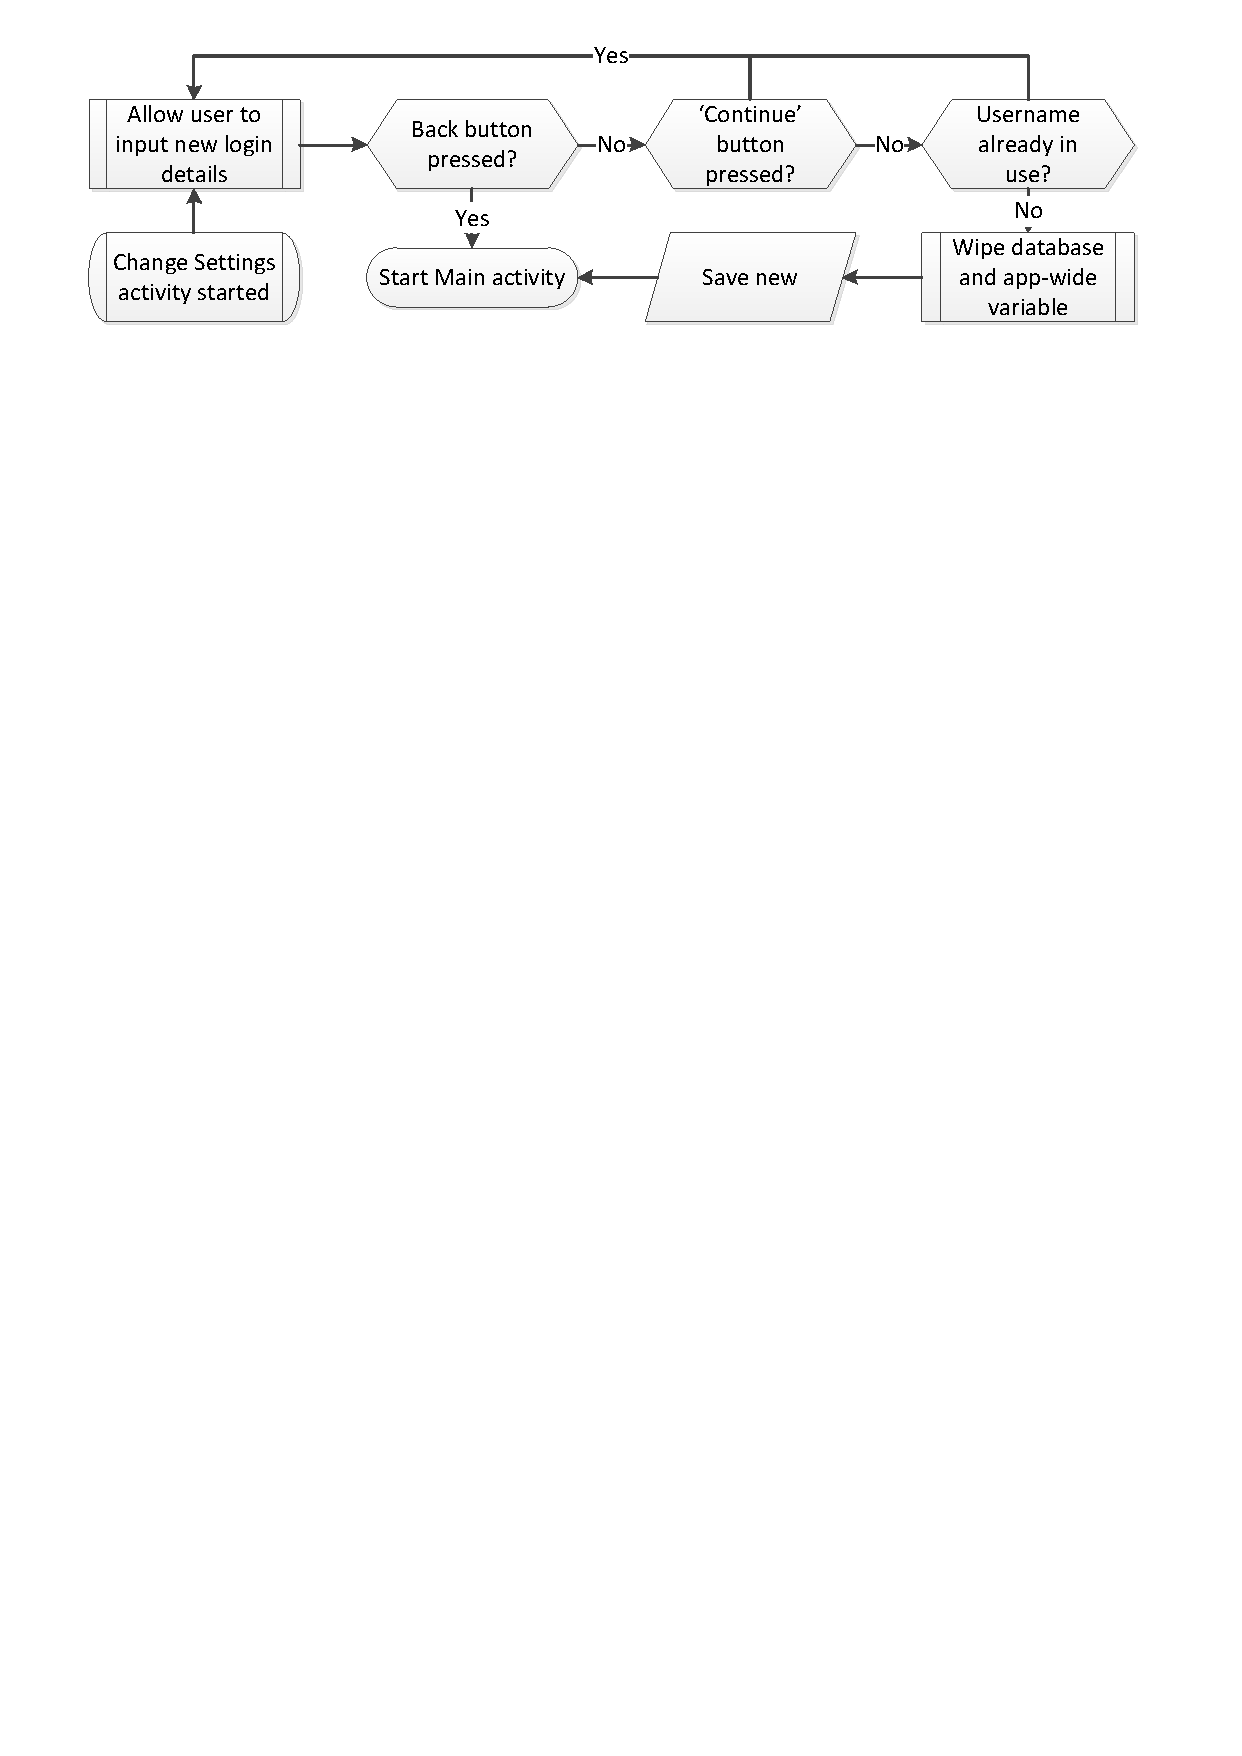
\includegraphics[clip = true, trim = 0 680 0 20,
 scale=0.7]{change_settings_processflow}
 \caption{The process flow of the Change Settings activity.}
 \label{fig:change-user-settings}
\end{figure}

\begin{figure}
 \centering 
 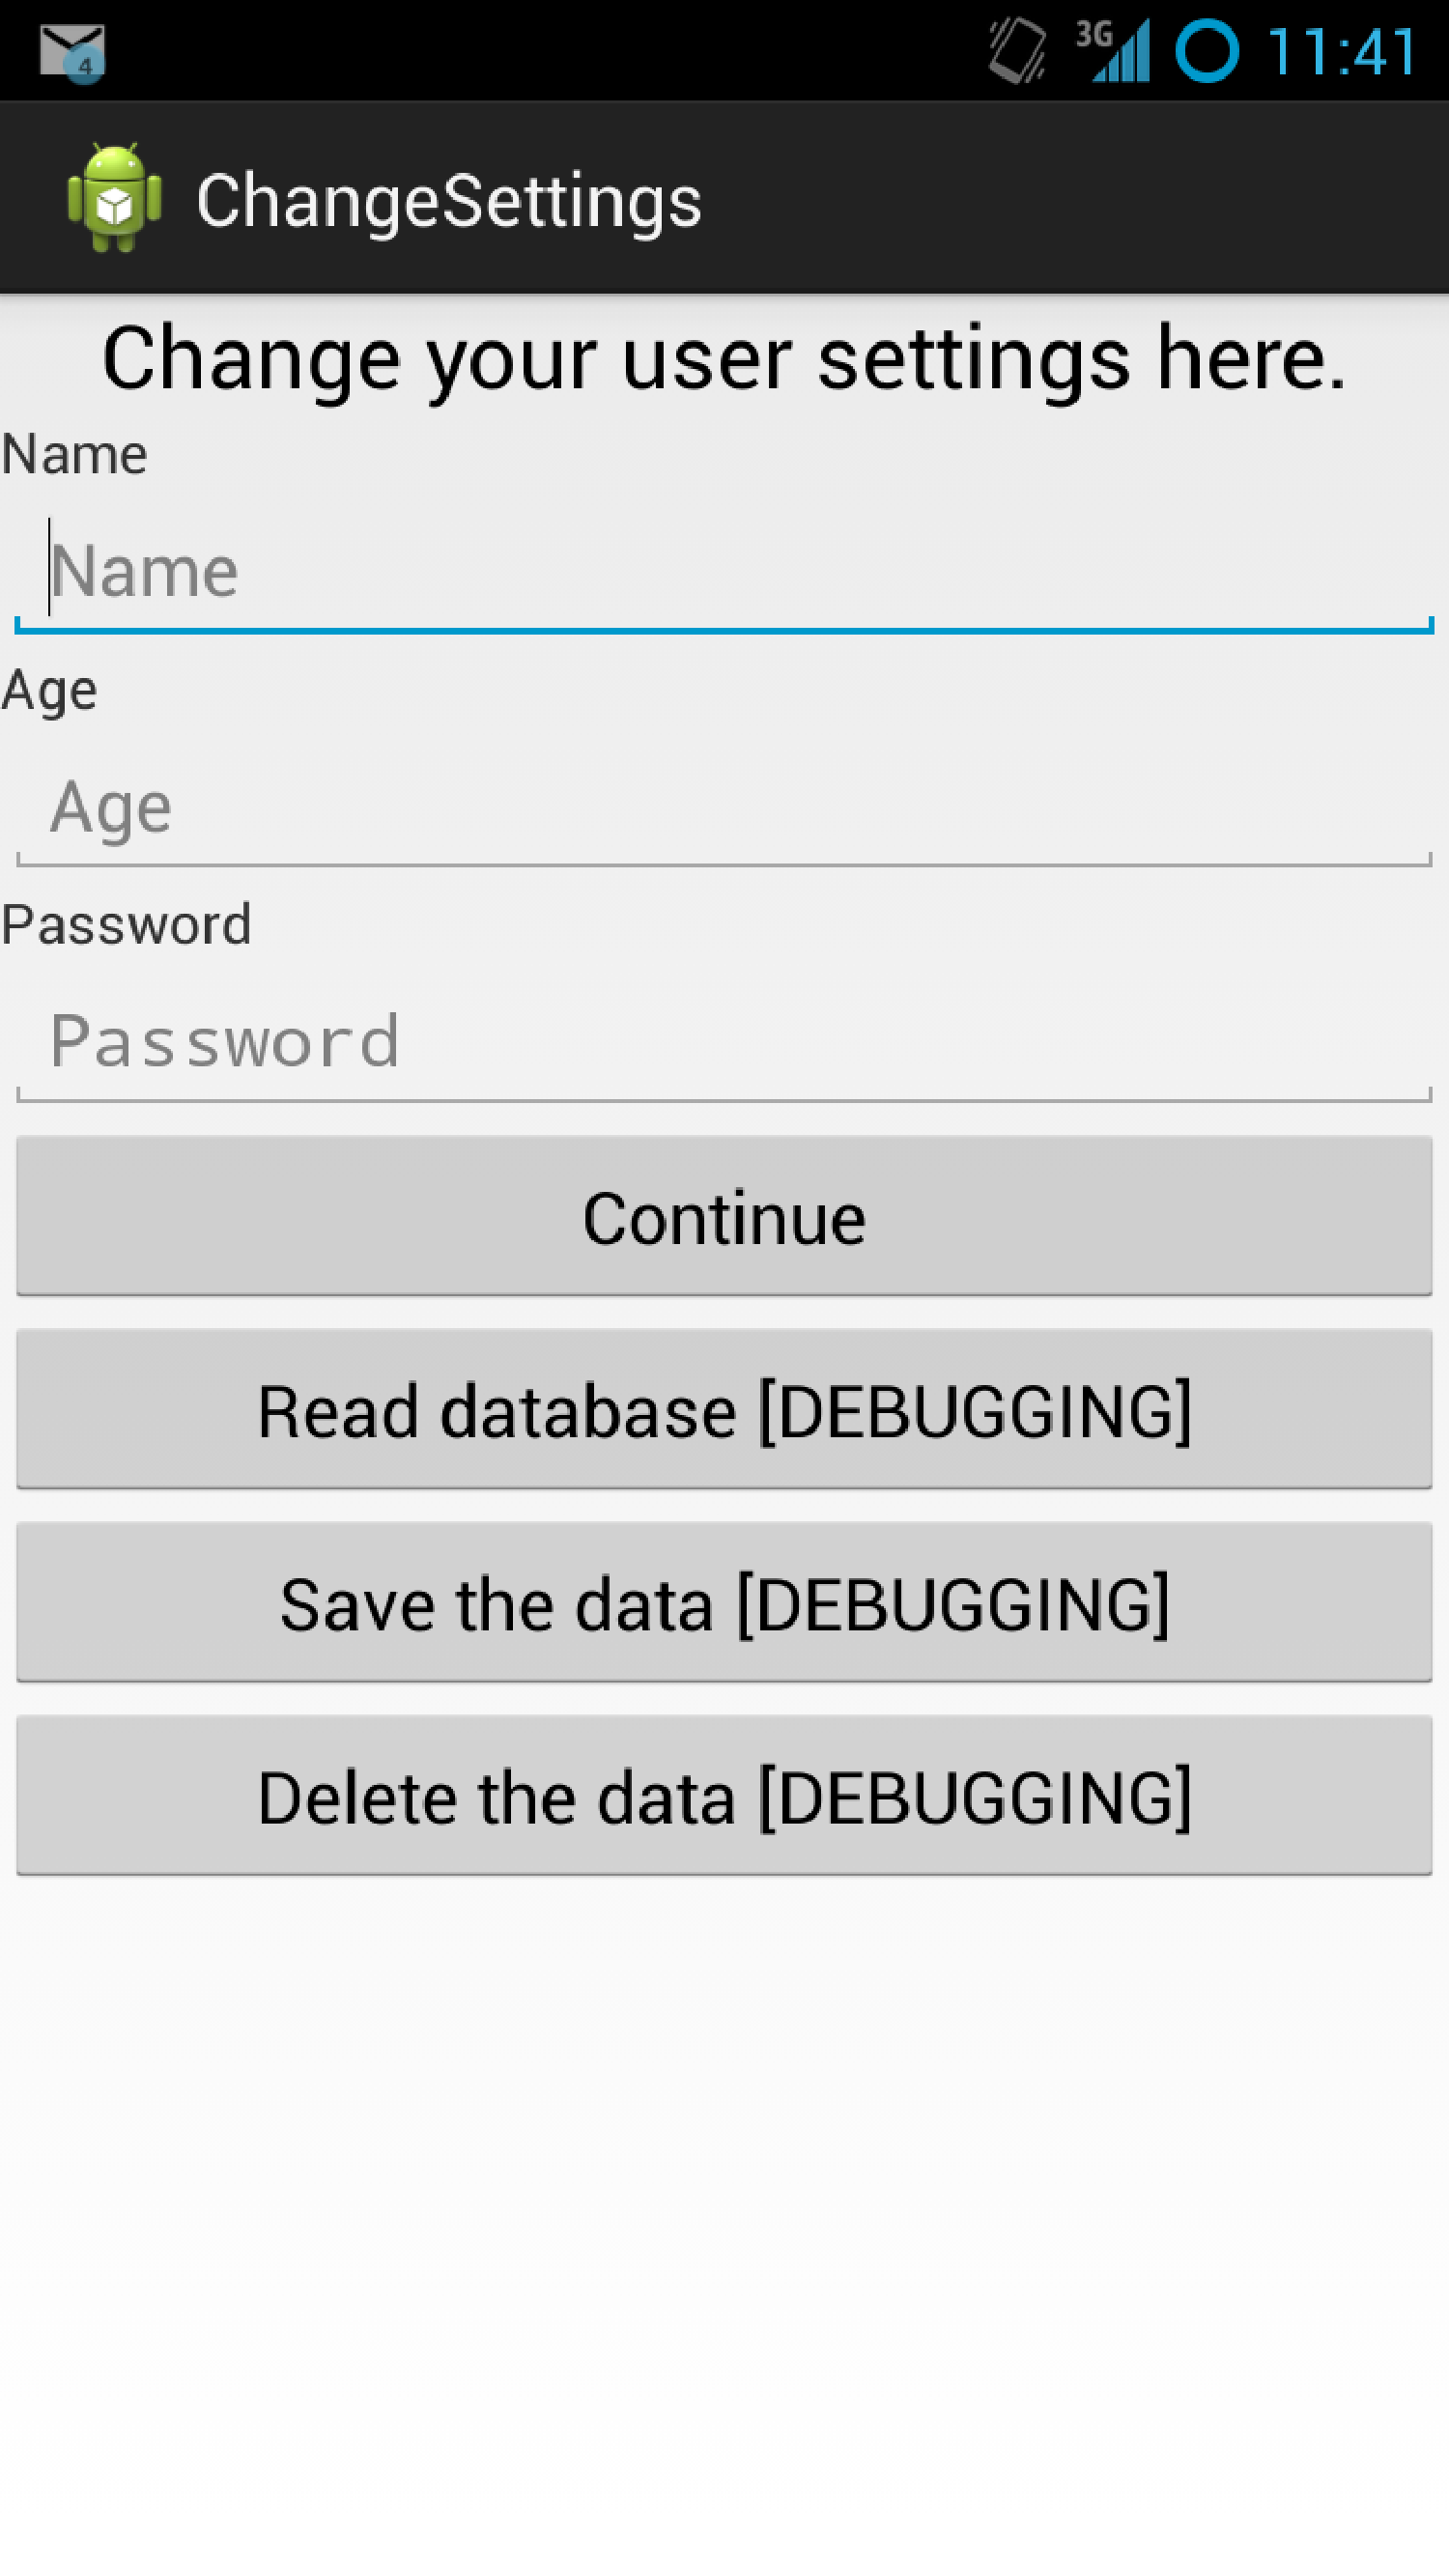
\includegraphics[clip = true, trim = 0 320 0 60,
 scale=0.2]{change_settings}
 \caption{A screenshot of the application's change settings activity.}
 \label{fig:change-settings-screenshot}
\end{figure}

When the application enters this activity, it prompts the user to enter his user
name and password. When the user presses the `continue button', the old database
entry and application-wide variable is overwritten with the new values the user entered.
The details stored on the server's database is not affected, however.

\subsection{Main Activity}

The main activity is the activity which is responsible for encrypting and
sending the purchase requests to the web server, receiving and decrypting
the purchase approval codes and sending the NFC messages to the VM's
NFC receiver. See Fig. \ref{fig:main-activity} for a process flow diagram
and Fig. \ref{fig:main-activity-screenshot} for a screenshot of this activity.

\begin{figure}
 \centering 
 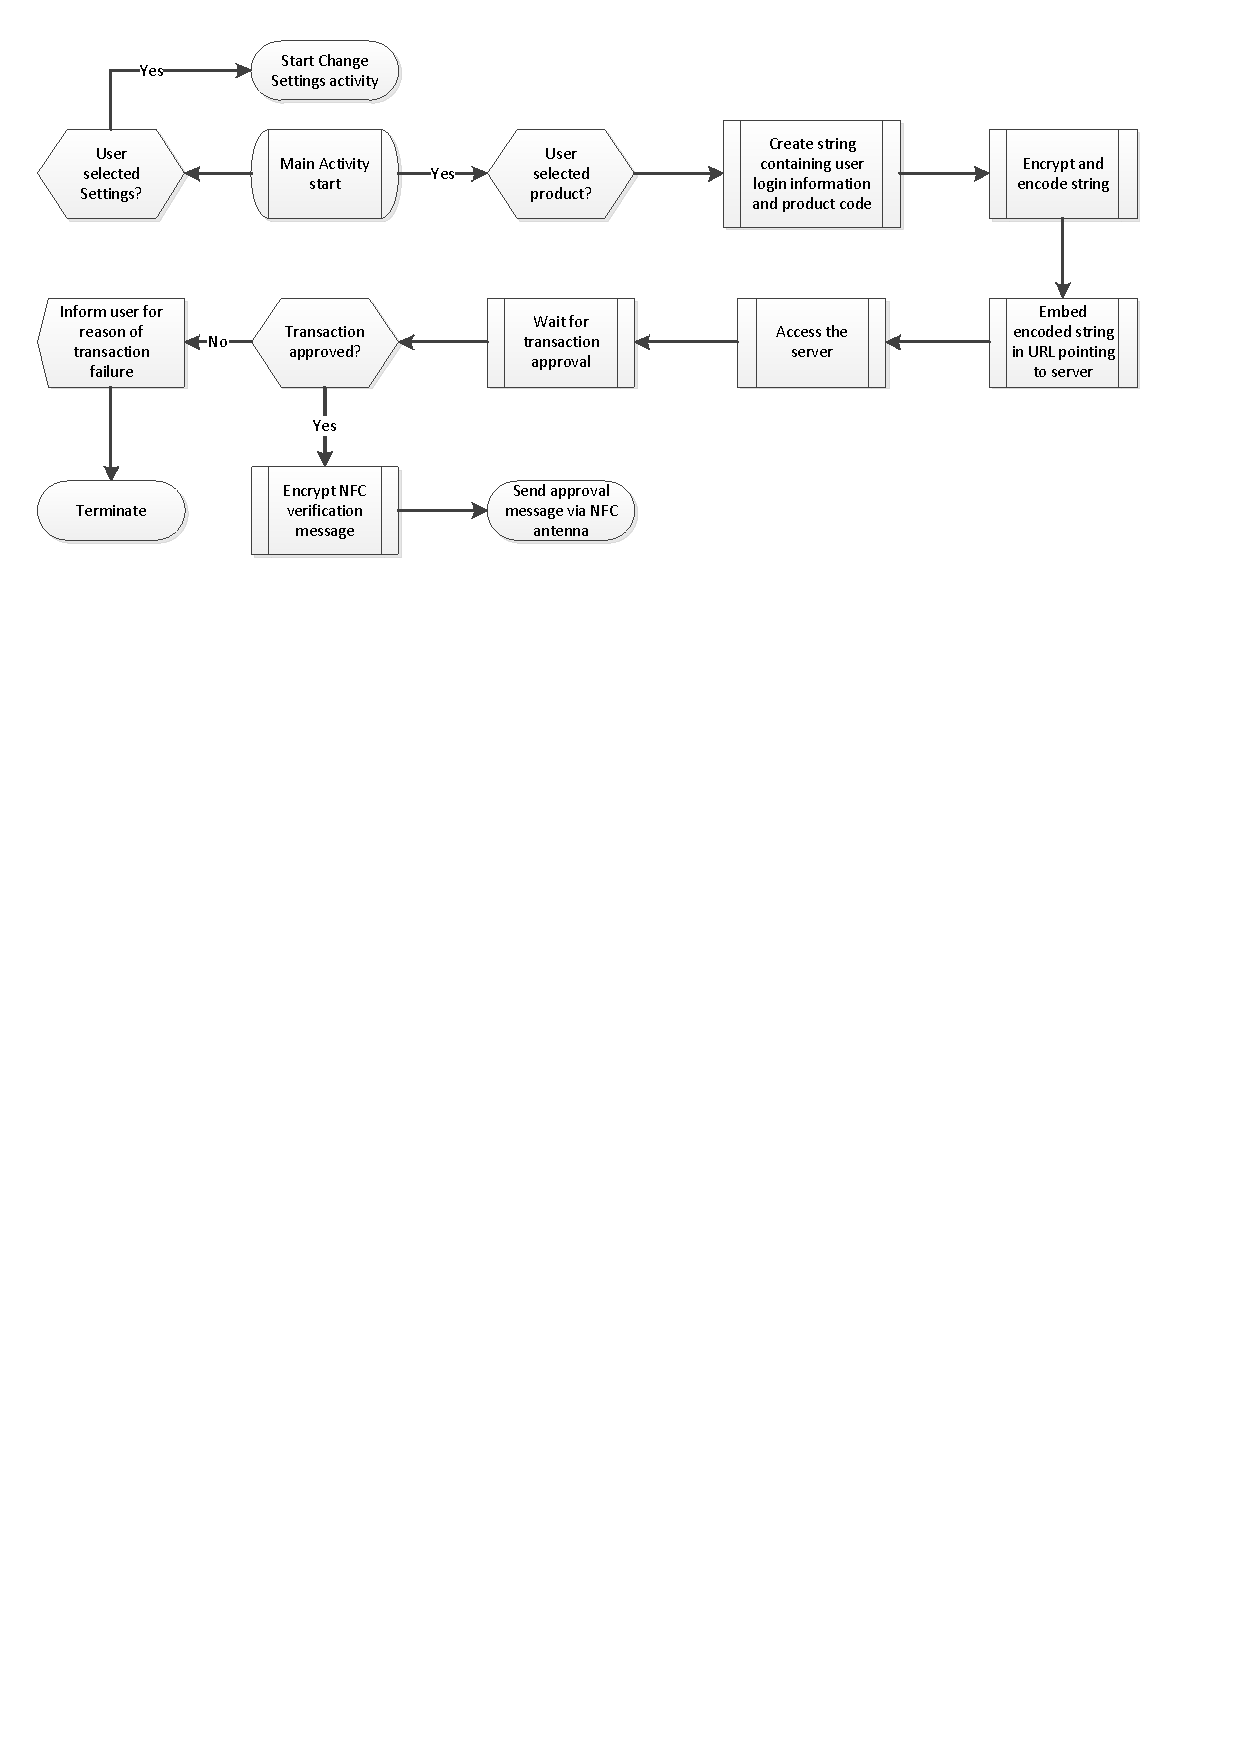
\includegraphics[clip = true, trim = 0 430 50 76,
 scale=0.7]{app_main_processflow}
 \caption{The process flow of the Main activity.}
 \label{fig:main-activity}
\end{figure}

\begin{figure}
 \centering 
 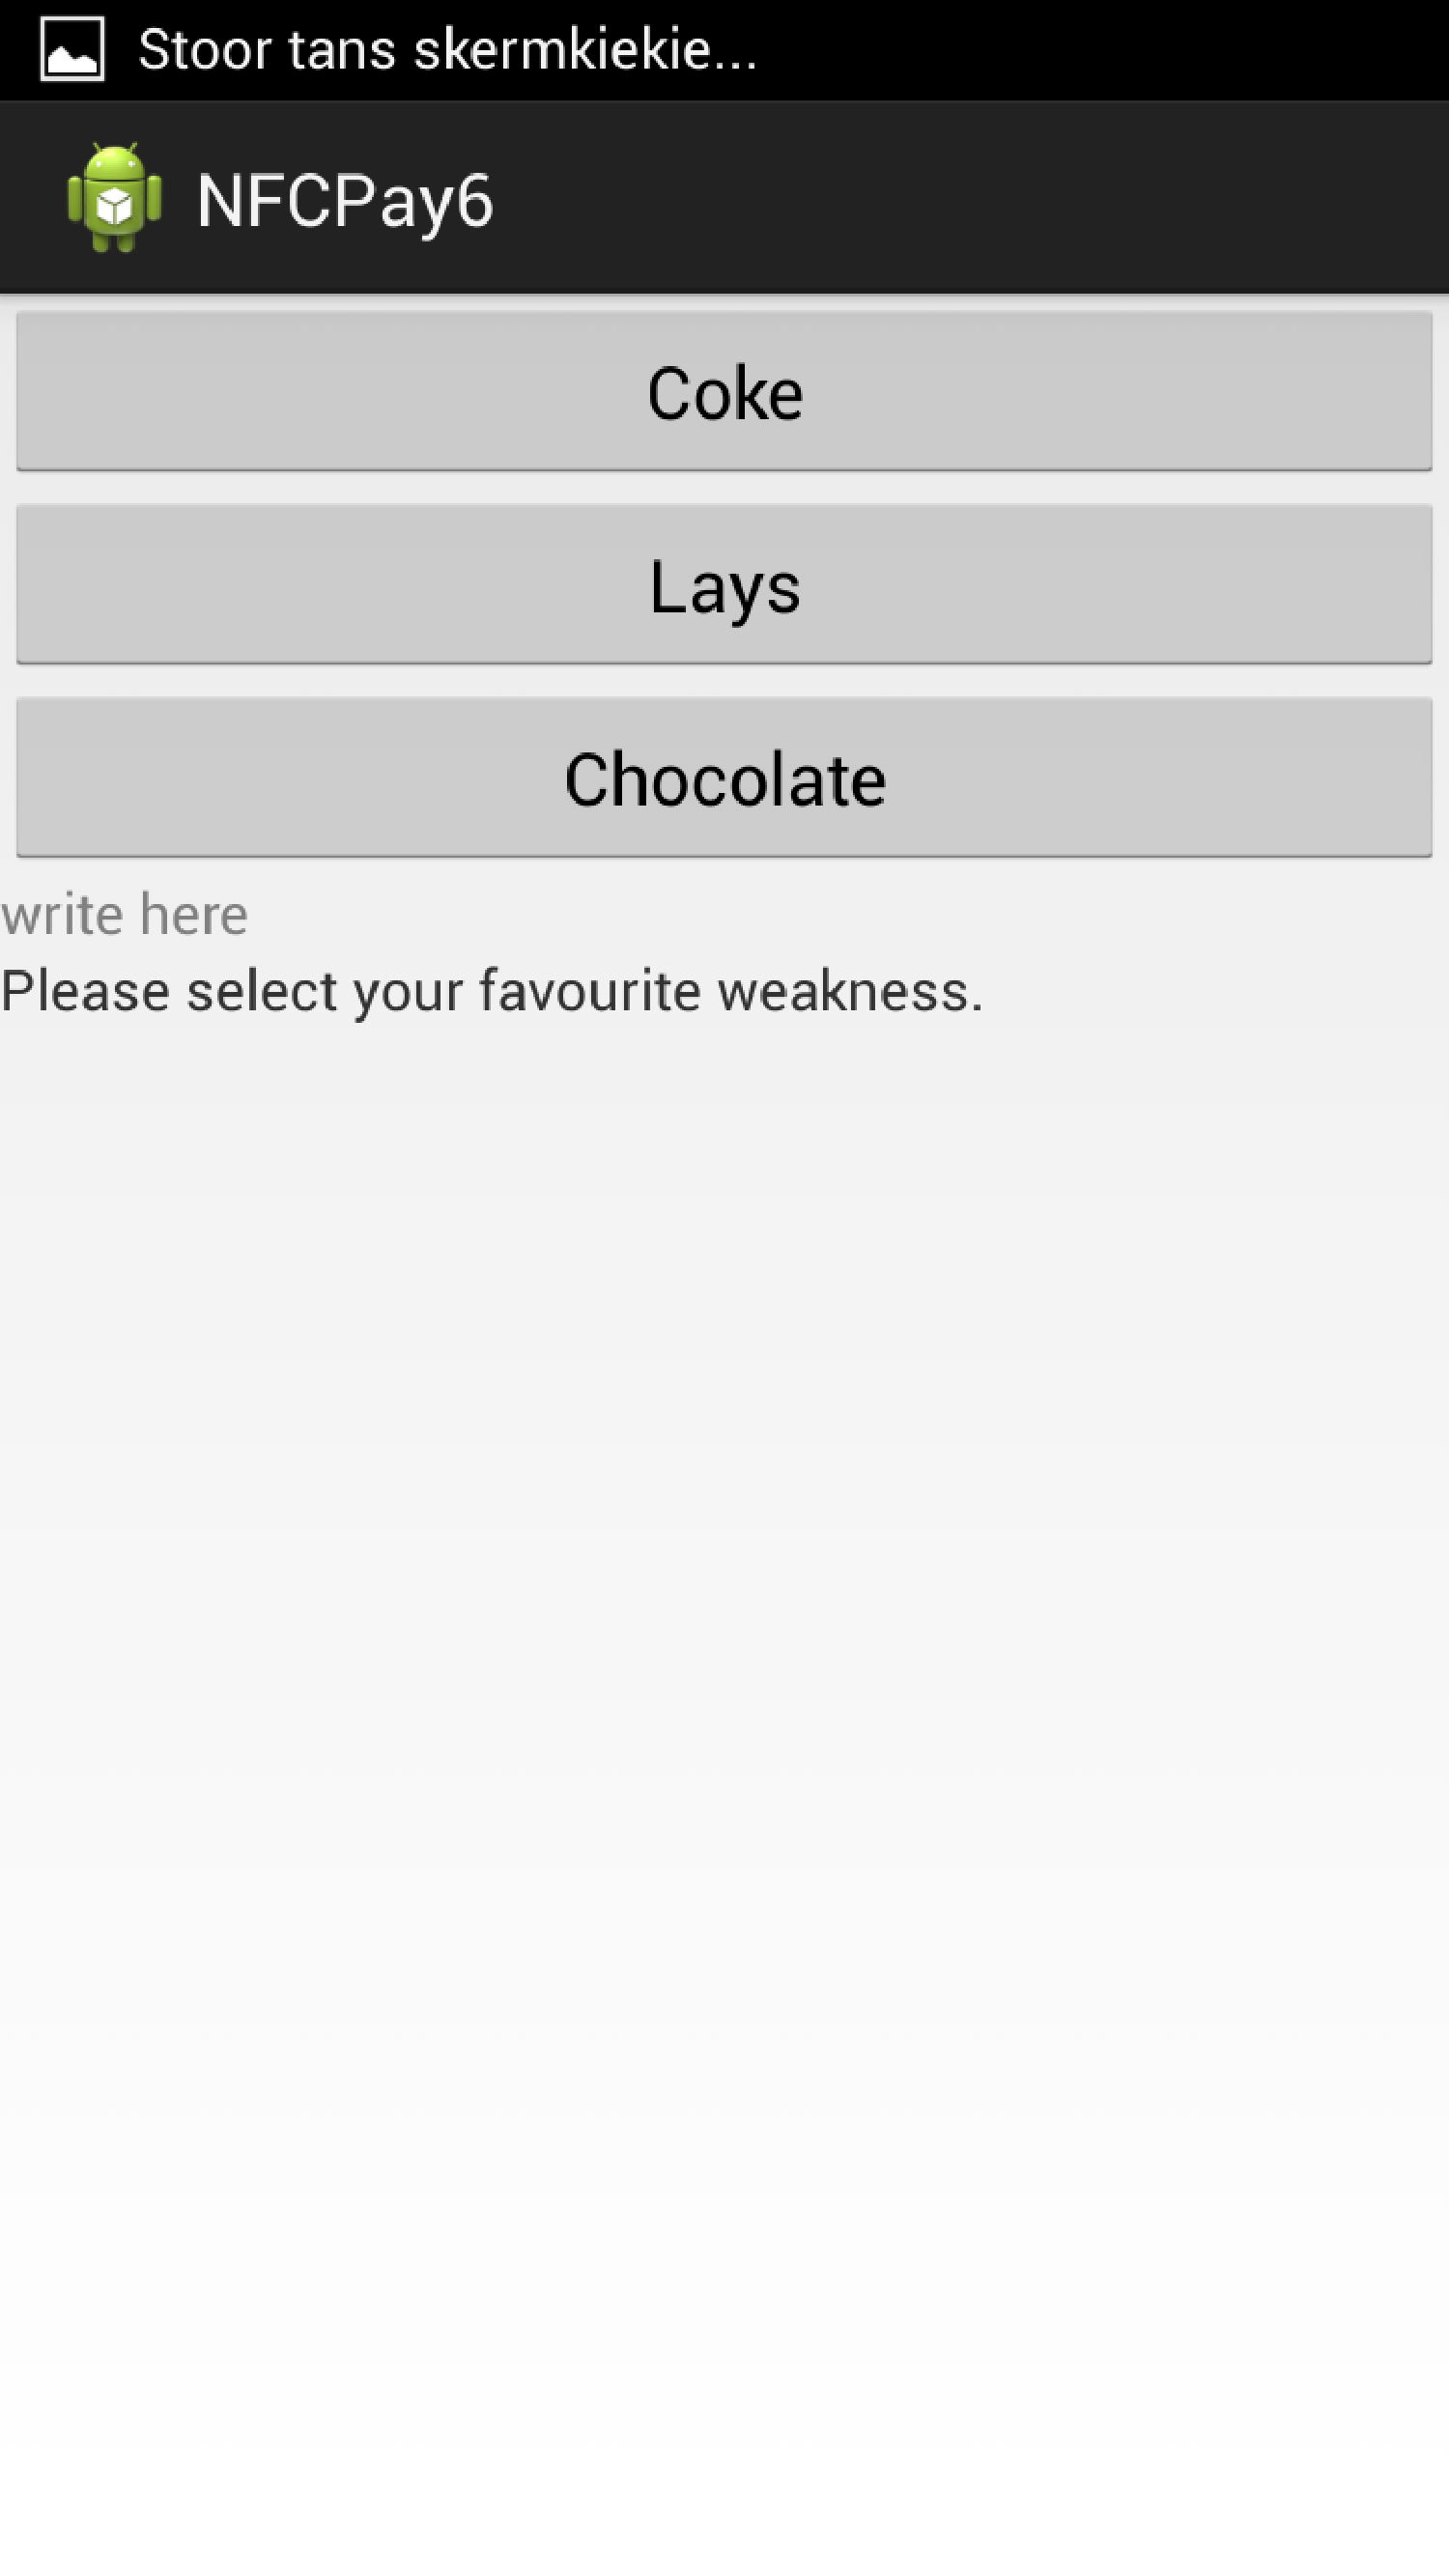
\includegraphics[clip = true, trim = 0 750 0 60,
 scale=0.2]{main_menu}
 \caption{A screenshot of the application's main activity.}
 \label{fig:main-activity-screenshot}
\end{figure}

As seen from Fig. \ref{fig:main-activity-screenshot}, the activity presents
the user with a list of products. When the user selects a product to buy, the
activity forms a data string by adding the product code, the user's login
name and password together. This data string is then encrypted with the
server's public key and then to base64. This encoded string
is then embedded inside a URL which points to the web server. 

The activity then requests this URL in the application's background, which prompts the
server to process the transaction (see Sec. \ref{sec:app-nfc} for more details on the
server's NFC processes). The server then tells the activity if the transaction
has been approved or denied. If it has been denied, the user is informed what was wrong. 
If it is approved, the activity activates the cellphone's NFC antenna which transmits an
encrypted approval message to the VM's NFC receiver.